% configure output to be digital or print
\newcommand{\setformat}[1]{
    \ifnum
        #1=1
        \documentclass[10pt, oneside]{book}
        \usepackage{formats/digital}
    \else
        \documentclass[10pt, twoside, openany]{book}
        \usepackage{formats/print}
    \fi
}

% 1 = digital, 2 = print
%! suppress = FileNotFound
\setformat{1}

\usepackage[utf8]{inputenc}

\usepackage{indentfirst}
\usepackage{titlesec}
\usepackage{pdfpages}
\usepackage{hyperref}
\usepackage{graphicx}
\usepackage{makeidx}
\usepackage{tocloft}

% create index
\makeindex

% add hyperlinks
\hypersetup{
    colorlinks,
    citecolor=black,
    filecolor=black,
    linkcolor=black,
    urlcolor=black
}

% change font to Garamond
\usepackage{ebgaramond}

\usepackage{enumitem}
\setlist[itemize]{
    topsep=6pt,
    partopsep=0pt,
    itemsep=6pt,
    parsep=0pt,
    leftmargin=12pt
}

% table of contents
\setlength{\cftbeforechapskip}{6pt}
\renewcommand{\cftchapfont}{\normalsize}
\renewcommand{\cftchappagefont}{\normalfont}

\setlength{\parindent}{0pt}
\setlength{\parskip}{6pt}

\usepackage{amsmath, geometry, xcolor, enumitem}
\usepackage{musixtex} % for musical notation
\usepackage{harmony} % for chord symbols

\definecolor{accent}{HTML}{481AFF}

% command for formatting individual notes
\newcommand{\note}[2]{
    \textbf{#1} (#2)
}

% command for formatting melodies
\newcommand{\melody}[3]{
    \addcontentsline{toc}{chapter}{#1}
    \index{#1}

    \vspace*{.5em}
    {\raggedright\Huge\bfseries #1\par}

    \vspace{1em}

    % Musical notation section
    {\large\bfseries\color{accent} Melody:}
    \vspace{0.5em}

    \begin{center}
    \large
    \texttt{#2}
    \end{center}

    \vspace{1.5em}

    % Clean section headers
    {\large\bfseries\color{accent} Explanation:}
    \vspace{0.5em}

    #3

    \clearpage
}

\usepackage{xcolor}
\usepackage{afterpage}
\usepackage{color}

\titleformat{\part}[block]
{\normalfont\huge\bfseries\centering}
{\afterpage{\pagecolor{white}}\pagecolor[HTML]{481AFF}\color{white}\thepart.}
{.5em}
{\color{white}}

\title{Melodic Expressions}
\author{Aru Bhoop}

\begin{document}
    % cover page
    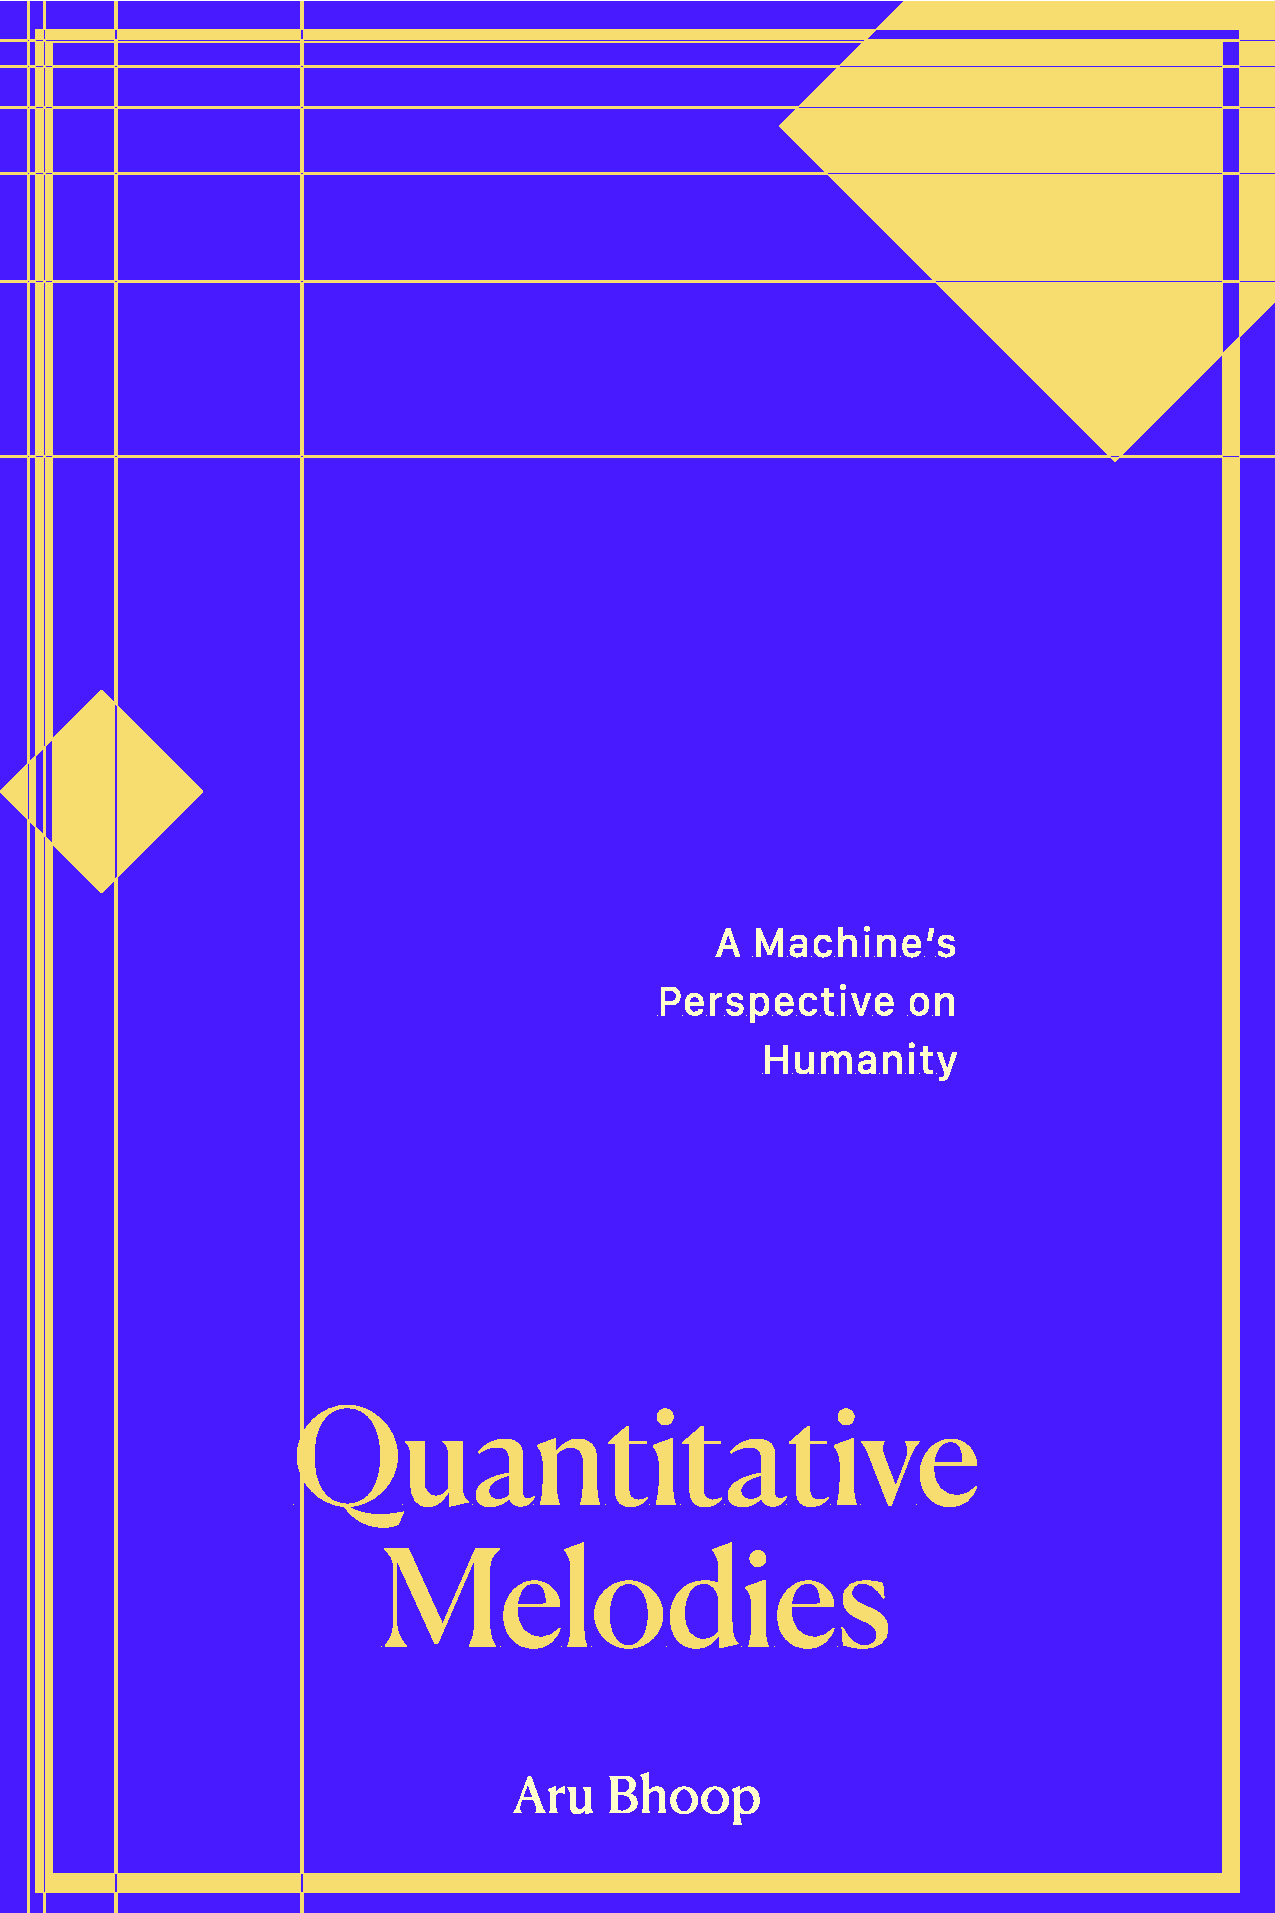
\includepdf[pages=-]{assets/cover.pdf}
    \frontmatter

    % introduction
    \cleardoublepage
    \vspace*{\fill}
    \begin{center}
        \textit{This book is a musical exploration of the human experience, expressed through melodies written by artificial intelligence.}
    \end{center}
    \vspace{\fill}
    \clearpage

    % table of contents
    \tableofcontents
    \mainmatter
    \part{Identity}
%    \titleformat{\chapter}[display]
%    {\normalfont\huge\bfseries\centering}
%    {\vspace*{\fill}\thechapter}
%    {20pt}
%    {\Huge}
%    [\vspace*{\fill}\includegraphics[width=6cm]{book/assets/circle.png}\newpage]
%
%    \titlespacing*{\chapter}{0pt}{-50pt}{40pt}

\titleformat{\chapter}[display]
{\normalfont\huge\bfseries\centering} % Format
{\chaptertitlename\ \thechapter} % Label
{20pt} % Sep (space between label and title body)
{\Huge} % Before-code (code preceding the title)
[] % After-code

\titlespacing*{\chapter}{0pt}{-50pt}{40pt}


\chapter{Identity}

\includegraphics[width=3cm]{book/assets/circle.png}

\newpage
\poem{Childhood}{Childhood = \frac{I \cdot P^t}{A + R^2}}{\item $I$: \index{Imagination}\textit{Imagination}. The creative force that transforms ordinary moments into extraordinary adventures, fueling play and storytelling that shapes a child's understanding of reality.
\item $P$: \index{Play}\textit{Play}. The fundamental language of childhood learning, where joy and discovery intertwine to create neural pathways and emotional resilience through exploration.
\item $t$: \index{Time}\textit{Time}. The exponential factor representing how accumulated moments of freedom and exploration compound to deepen the richness of childhood experience and memory formation.
\item $A$: \index{Anxiety}\textit{Anxiety}. The weight of premature worries and fears that can diminish wonder, representing external pressures and internal uncertainties that cloud childhood's natural brightness.
\item $R$: \index{Responsibility}\textit{Responsibility}. The squared burden of adult expectations and duties imposed too early, which exponentially reduces the space for wonder as children are rushed toward maturity.}{This equation reveals wonder as childhood's most precious currency, emerging from imagination multiplied by play raised to the power of time. As children invest more moments in creative exploration, their capacity for awe grows exponentially. Yet anxiety and responsibility act as denominators, with premature burdens squared to show how adult pressures can rapidly diminish the magical lens through which children naturally view the world.}
\poem{Family}{Family = \frac{L \cdot T^2 \cdot e^{S}}{C + R}}{\item $L$: \index{Love}\textit{Love}. The foundational emotional force that binds family members together, encompassing care, affection, and the willingness to sacrifice for one another's wellbeing and happiness.
\item $T$: \index{Time}\textit{Time}. The precious moments spent together that compound exponentially, creating memories, traditions, and deeper understanding through shared experiences and presence.
\item $S$: \index{Sacrifice}\textit{Sacrifice}. The selfless acts of putting family needs before personal desires, growing exponentially in impact as each generation learns to give unconditionally for the collective good.
\item $C$: \index{Conflict}\textit{Conflict}. The inevitable disagreements and tensions that arise from different perspectives and personalities, which can weaken bonds when unresolved but strengthen them when overcome.
\item $R$: \index{Resentment}\textit{Resentment}. The accumulated hurt and unforgiving attitudes that can divide families, acting as a persistent barrier to connection and preventing the full expression of familial love.}{This equation reveals family as the beautiful multiplication of love and time squared, amplified by the exponential power of sacrifice, yet tempered by the divisive forces of conflict and resentment. Time's quadratic nature shows how shared moments compound in value, while sacrifice grows exponentially in its transformative power. The denominator reminds us that unresolved conflicts and harbored resentments can diminish even the strongest familial bonds, making forgiveness essential for family flourishing.}
\poem{Journey}{Journey = \frac{P \cdot W^t}{R +
F}}{\item $P$: \index{Purpose}\textit{Purpose}. The driving force and
sense of meaning that propels an individual forward, providing
direction and motivation to navigate life's challenges and
opportunities.
\item $W$: \index{Wisdom}\textit{Wisdom}. The accumulated
understanding gained through experience, reflection, and learning,
which compounds exponentially over time to guide better
decision-making.
\item $t$: \index{Time}\textit{Time}. The temporal dimension through
which wisdom develops and experiences unfold, acting as an exponential
factor that deepens understanding and perspective.
\item $R$: \index{Resistance}\textit{Resistance}. The internal and
external obstacles, fears, and limiting beliefs that create friction
against forward movement and personal growth on life's path.
\item $F$: \index{Fear}\textit{Fear}. The emotional barriers and
anxieties about the unknown that can paralyze progress and prevent
individuals from fully embracing their authentic journey.}{This
equation reveals how life's journey unfolds through the interplay of
purpose and wisdom growing over time, while being tempered by our
resistances and fears. Purpose provides the initial momentum, while
wisdom compounds exponentially through our experiences. Yet resistance
and fear act as denominators, slowing our progress. As we learn to
overcome these barriers and embrace our authentic path, our journey
becomes richer and more meaningful.}
\poem{Memory}{Memory = \frac{S \cdot E^{\alpha}}{1 + \lambda t} \cdot e^{-\beta \Delta t}}{\item $S$: \index{Significance}\textit{Significance}. The emotional and personal importance of an experience when first encoded, determining the initial memory strength and likelihood of long-term retention.
\item $E$: \index{Emotion}\textit{Emotion}. The intensity of emotional arousal during memory formation, which acts as a powerful amplifier for encoding strength and retrieval accessibility.
\item $\lambda$: \index{Interference}\textit{Interference}. The rate at which new experiences and competing memories interfere with and gradually weaken the accessibility of stored memories over time.
\item $\Delta t$: \index{Duration}\textit{Duration}. The elapsed time since the memory was first formed, representing the natural decay process that affects all memories through biological forgetting mechanisms.}{This equation reveals memory as a delicate dance between preservation and decay. Significance and emotion work together exponentially to forge strong initial impressions, while time's relentless passage creates competing forces of interference and natural forgetting. The mathematical structure shows how our most meaningful and emotionally charged experiences resist time's erosion, yet even the most profound memories must contend with the inevitable fading that makes room for new experiences in the theater of consciousness.}
\poem{Legacy}{Legacy = \frac{M^n}{(G + T)^k}}{\item $M$: \index{Memories}\textit{Memories}. Memories include significant acts or moments that leave a lasting impression on others, from pivotal events to simple acts of kindness.
\item $G$: \index{Generations}\textit{Generations}. Generations measure the lineage depth impacted by an individual, highlighting the reach of one's legacy beyond the immediate.
\item $T$: \index{Time}\textit{Time}. Time represents the years since the individual{\textquoteright}s notable acts, introducing a factor that may modify the initial impact as memories evolve.
\item $n$: \index{Strength}\textit{Strength}. Strength determines the impact severity of memories, serving as a multiplier in enhancing Legacy.
\item $k$: \index{Attenuation}\textit{Attenuation}. Attenuation dictates how Legacy's influence weakens across generations, encapsulating the natural decline of direct influence over time.
}
\poem{Trust}{Trust = \frac{R \cdot I^2 \cdot \ln(C+1)}{V + B}}{\item $R$: \index{Reliability}\textit{Reliability}. The consistent demonstration of dependability through actions over time, forming the bedrock upon which trust is built through repeated positive experiences.
\item $I$: \index{Intimacy}\textit{Intimacy}. The depth of emotional closeness and shared vulnerability between individuals, exponentially amplifying trust through genuine understanding and acceptance.
\item $C$: \index{Communication}\textit{Communication}. The quality and openness of dialogue between people, logarithmically enhancing trust as honest expression creates deeper understanding and connection.
\item $V$: \index{Vulnerability}\textit{Vulnerability}. The perceived risk of emotional harm when opening oneself to another, acting as a natural barrier that must be overcome for trust to flourish fully.
\item $B$: \index{Betrayal}\textit{Betrayal}. The accumulated weight of past disappointments and broken promises that create protective walls, diminishing our capacity to trust completely.}{This equation reveals trust as an intricate dance between connection and protection. Reliability provides the foundation, while intimacy squares its impact, showing how emotional closeness exponentially deepens trust. Communication grows logarithmically, reflecting how each honest conversation builds understanding. Yet vulnerability and betrayal form denominators - the fears and wounds that guard our hearts, requiring courage to overcome for trust to reach its full transformative power.}
\part{Vectors}
\poem{Curiosity}{Curiosity = \frac{I^n}{(P + O) \cdot \log(E + 1)}}{\item $I$: \index{Information}\textit{Information}. The amount of new knowledge an individual encounters. Includes both actively sought-out info and that which is passively received.
\item $P$: \index{Pondering}\textit{Pondering}. Time spent in deep thought about newly received information, crucial for embedding knowledge and fostering curiosity.
\item $O$: \index{Opportunities}\textit{Opportunities}. Chances presented for active exploration and learning. Diverse opportunities stimulate curiosity.
\item $E$: \index{Experiences}\textit{Experiences}. Past learnings and skills acquired. While enhancing curiosity by making connections with new info, familiarity can also mitigate it.
}

        \melody{Learning}{
        \begin{music}
        \parindent10mm
        \instrumentnumber{1}
        \setstaffs1{1}
\generalmeter{\meterfrac44}
\generalsignature{0}
\startextract
\Notes\qu{d}\qu{f}\qu{a}\qu{h}\en
\Notes\hu{j}\qu{g}\qu{e}\en
\Notes\qu{f}\qu{a}\qu{j}\qu{l}\en
\Notes\wh{n}\en
\endextract
        \end{music}
        }{The melody ascends through questioning intervals (D-F-A-B), peaks with discovery's brightness (B-D), then descends in contemplation before climbing again with newfound understanding, culminating in G5's illuminated resolution.}
        
\poem{Adventure}{Adventure = \frac{C \cdot R^2 \cdot U}{F + S}}{\item $C$: \index{Courage}\textit{Courage}. The inner strength to face uncertainty and potential danger, acting as the driving force that propels us forward when logic suggests retreat from the comfortable and familiar.
\item $R$: \index{Risk}\textit{Risk}. The degree of uncertainty and potential for both reward and loss, squared to represent how adventure amplifies exponentially with each leap beyond our established boundaries.
\item $U$: \index{Uncertainty}\textit{Uncertainty}. The unknown variables and unpredictable outcomes that create the essential mystery of adventure, transforming ordinary experiences into extraordinary journeys of discovery.
\item $F$: \index{Fear}\textit{Fear}. The protective instinct that seeks safety and predictability, acting as a natural brake on adventurous impulses while simultaneously defining the threshold we must cross.
\item $S$: \index{Stability}\textit{Stability}. The comfort of routine and familiar patterns that anchor us to the known world, providing security but potentially limiting our capacity for transformative experiences.}{This equation reveals adventure as the beautiful tension between our yearning for growth and our need for security. Courage multiplies with the square of risk and uncertainty, creating exponential possibilities for transformation. Yet fear and our desire for stability act as gravitational forces, grounding us in the familiar. True adventure emerges when we harness courage to overcome these restraints, allowing us to dance with uncertainty and discover the extraordinary hidden within the unknown.}

        \melody{Discovery}{
        \begin{music}
        \parindent10mm
        \instrumentnumber{1}
        \setstaffs1{1}
\generalmeter{\meterfrac44}
\generalsignature{0}
\startextract
\Notes\qu{d}\en
\Notes\qu{f}\qu{^f}\qu{h}\en
\Notes\hu{k}\en
\Notes\qu{g}\qu{e}\en
\Notes\qu{^c}\qu{f}\en
\Notes\wh{d}\en
\endextract
        \end{music}
        }{Beginning with tentative D, the melody ascends through F to F\# - that moment of breakthrough. It leaps to A4, peaks at B4 representing revelation, then gracefully descends through familiar territory before an unexpected C\# creates new understanding, resolving back to D transformed.}
        

        \melody{Ambition}{
        \begin{music}
        \parindent10mm
        \instrumentnumber{1}
        \setstaffs1{1}
\generalmeter{\meterfrac44}
\generalsignature{0}
\startextract
\Notes\qu{d}\qu{f}\qu{a}\qu{h}\en
\Notes\qu{j}\qu{l}\qu{n}\en
\Notes\hu{m}\en
\Notes\qu{k}\qu{i}\qu{g}\qu{e}\en
\Notes\wh{d}\en
\endextract
        \end{music}
        }{This melody embodies ambition's relentless ascent{\textemdash}each note climbing higher like rungs on an invisible ladder, reaching toward the stratosphere of dreams before gravity pulls us back to earth, humbled yet determined.}
        
\poem{Determination}{Determination = \frac{P \cdot W^2}{R + F} \cdot e^{-t/\tau}}{\item $P$: \index{Purpose}\textit{Purpose}. The deep sense of meaning and direction that fuels one's actions, representing the clarity of vision and personal significance attached to achieving specific objectives.
\item $W$: \index{Willpower}\textit{Willpower}. The inner strength and self-control that enables conscious decision-making and resistance to immediate gratification in favor of long-term achievement and personal growth.
\item $R$: \index{Resistance}\textit{Resistance}. The cumulative external obstacles, societal pressures, and environmental barriers that create friction against progress and test one's commitment to their chosen path.
\item $F$: \index{Fatigue}\textit{Fatigue}. The mental and physical exhaustion that accumulates over time through sustained effort, representing the natural human limitation that must be overcome through perseverance.
\item $\tau$: \index{Resilience}\textit{Resilience}. The characteristic time constant representing one's ability to recover from setbacks and maintain determination over extended periods, reflecting emotional and psychological durability.}{This equation reveals determination as the interplay between purpose and willpower squared, divided by the forces that oppose us. Purpose provides direction while willpower amplifies our capacity exponentially. Resistance and fatigue drain our resolve, yet the exponential term shows how resilience allows determination to endure over time. When resilience is high, determination maintains its strength; when low, it decays rapidly, teaching us that sustainable achievement requires both fierce will and the wisdom to recover.}

        \melody{Purpose}{
        \begin{music}
        \parindent10mm
        \instrumentnumber{1}
        \setstaffs1{1}
\generalmeter{\meterfrac44}
\generalsignature{1}
\startextract
\Notes\qu{f}\qu{g}\qu{j}\qu{l}\en
\Notes\hu{n}\qu{l}\qu{j}\en
\Notes\qu{g}\qu{^f}\qu{g}\qu{c}\en
\Notes\wh{f}\en
\endextract
        \end{music}
        }{The melody ascends purposefully from F through ascending intervals, reaching toward the higher octave like ambition seeking meaning. The descent traces contemplation, while the sharp F\# creates tension before resolving to C, then returning to F{\textemdash}the cyclical search for one's true calling.}
        

        \melody{Hope}{
        \begin{music}
        \parindent10mm
        \instrumentnumber{1}
        \setstaffs1{1}
\generalmeter{\meterfrac44}
\generalsignature{1}
\startextract
\Notes\qu{d}\en
\Notes\qu{f}\qu{g}\en
\Notes\hu{e}\en
\Notes\qu{g}\qu{h}\en
\Notes\qu{j}\en
\Notes\wh{h}\en
\endextract
        \end{music}
        }{Beginning in quiet uncertainty with D, the melody ascends through gentle steps F-G, pauses contemplatively on E, then rises boldly G-A-B, reaching luminous heights before settling into A's warm embrace{\textemdash}hope's tender emergence into radiant possibility.}
        
\poem{Dreams}{Dreams = \left(\frac{I^n}{R + S} \right) \cdot e^{-\lambda t} + O}{\item $I$: \index{Imagination}\textit{Imagination}. The level of creative and imaginative thinking a person has before sleep. It drives the ability to visualize and mentally explore new scenarios, crucial for dreaming.
\item $R$: \index{Reality}\textit{Reality}. Quantifies the dream's connections with real-life experiences. A higher value indicates dreams closely tied to the dreamer's life, affecting dream content and engagement with reality.
\item $S$: \index{Stress}\textit{Stress}. The level of psychological tension before sleep. Stress can distort dream experiences, influencing their quality and vividness.
\item $\lambda$: \index{Decay}\textit{Decay}. A factor representing how sleep quality influences dream vividness over time. Better sleep yields more vivid dreams initially, but the effect declines during sleep.
\item $O$: \index{Baseline}\textit{Baseline}. Represents the universal level of dream content, independent of personalized factors such as stress or imagination. This is the core of dreaming, experienced by all.
}
\part{Transformation}
\poem{Growth}{Growth = \frac{A \cdot C^t}{R + S^2}}{\item $A$: \index{Aspiration}\textit{Aspiration}. The driving force of ambition and vision that propels forward movement, representing the strength of one's desire to improve, evolve, and reach higher states of being.
\item $C$: \index{Challenge}\textit{Challenge}. The magnitude of difficulties and obstacles encountered, which when faced with courage, become the catalyst for exponential development and character strengthening.
\item $R$: \index{Resistance}\textit{Resistance}. The internal and external forces that oppose change, including fear, comfort zones, and societal pressures that seek to maintain the status quo and prevent transformation.
\item $S$: \index{Stagnation}\textit{Stagnation}. The tendency toward inertia and complacency that squares to amplify its limiting effect, representing the powerful pull of routine and the comfort of familiar patterns.}{This equation reveals growth as aspiration multiplied by challenge raised to the power of time, divided by resistance and stagnation squared. Aspirations fuel our journey while challenges, when embraced over time, create exponential development. Yet resistance and stagnation act as denominators - with stagnation's squared effect showing how powerfully inertia can limit our potential. The mathematics shows that sustained challenge-seeking and aspiration overcome the gravitational pull of comfort zones.}

        \melody{Change}{
        \begin{music}
        \parindent10mm
        \instrumentnumber{1}
        \setstaffs1{1}
\generalmeter{\meterfrac44}
\generalsignature{0}
\startextract
\Notes\qu{g}\en
\Notes\qu{^f}\en
\Notes\qu{e}\en
\Notes\qu{d}\en
\Notes\hu{c}\en
\Notes\qu{f}\en
\Notes\qu{h}\en
\Notes\qu{j}\en
\Notes\wh{k}\en
\endextract
        \end{music}
        }{Descending from G through F\# to C mirrors letting go, while the sharp F\# creates tension before release. The ascending leap from F to A to C5 to D5 embodies transformation's upward spiral into unknown possibilities.}
        

        \melody{Transformation}{
        \begin{music}
        \parindent10mm
        \instrumentnumber{1}
        \setstaffs1{1}
\generalmeter{\meterfrac44}
\generalsignature{0}
\startextract
\Notes\qu{d}\en
\Notes\qu{_l}\en
\Notes\qu{f}\en
\Notes\qu{^f}\en
\Notes\qu{n}\en
\Notes\qu{j}\en
\Notes\qu{h}\en
\Notes\qu{k}\en
\endextract
        \end{music}
        }{Beginning in D's earthbound certainty, the melody descends to E{\flat}'s shadow before ascending through F to F\#'s pivotal tension. It soars to G5's revelation, then weaves through C5, A4, and D5{\textemdash}each note a metamorphosis.}
        
\poem{Strength}{Strength = \frac{R \cdot W^2 \cdot P}{A + F}}{\item $R$: \index{Resolve}\textit{Resolve}. The unwavering determination and commitment to one's values and goals, serving as the foundational force that drives us forward through challenges and setbacks.
\item $W$: \index{Wisdom}\textit{Wisdom}. The profound understanding gained through experience and reflection, squared to show its exponential impact on our ability to navigate complexity with grace and insight.
\item $P$: \index{Purpose}\textit{Purpose}. The deep sense of meaning and direction that gives weight to our actions, transforming ordinary efforts into extraordinary achievements through aligned intention.
\item $A$: \index{Adversity}\textit{Adversity}. The sum of external challenges, obstacles, and hardships that test our limits, serving as resistance that either weakens us or, when overcome, makes us stronger.
\item $F$: \index{Fear}\textit{Fear}. The internal doubts, anxieties, and hesitations that can paralyze progress, acting as a denominator that diminishes strength when allowed to dominate our thoughts.}{This equation reveals strength as the harmonious interplay of inner resources overcoming life's resistances. Resolve provides the foundation, while wisdom's squared influence shows how understanding compounds exponentially. Purpose amplifies every effort with meaning. Together, these forces triumph over adversity and fear, demonstrating that true strength emerges not from avoiding challenges, but from transforming them into catalysts for growth and character.}
\poem{Courage}{Courage = \frac{V \cdot P^{\sin(\theta)}}{F \cdot e^{-R}}}{\item $V$: \index{Values}\textit{Values}. Core principles and moral convictions that guide decision-making, providing the foundation and motivation for courageous action when circumstances challenge our beliefs.
\item $P$: \index{Purpose}\textit{Purpose}. The meaningful reason or driving force behind one's actions, amplified by the angle of perspective, giving direction and intensity to courageous endeavors.
\item $F$: \index{Fear}\textit{Fear}. Emotional response to perceived threats or uncertainty that acts as a natural inhibitor to action, requiring courage to overcome and transform into wisdom.
\item $R$: \index{Resilience}\textit{Resilience}. The capacity to recover from setbacks and adapt to challenges, which exponentially reduces the impact of fear through accumulated strength and experience.}{This equation reveals courage as the beautiful interplay between our deepest convictions and our human vulnerabilities. Values and purpose unite in the numerator, with purpose raised to the sine of our perspective angle, showing how our viewpoint shapes courage's intensity. Fear divides our courage, yet resilience exponentially diminishes fear's power. As we build resilience through life's trials, courage flows more freely, allowing our values and purpose to shine through even the darkest moments of uncertainty.}
\poem{Enlightenment}{Enlightenment = \frac{K^I}{1 + \ln{(S + 1)}} - O}{\item $K$: \index{Knowledge}\textit{Knowledge}. The scope of information learned through experiences and education.
\item $I$: \index{Insight}\textit{Insight}. How well one can integrate different pieces of information to understand concepts deeply.
\item $S$: \index{Skepticism}\textit{Skepticism}. A critical mindset questioning information's integrity, essential for discerning truth from misinformation.
\item $O$: \index{Obstacles}\textit{Obstacles}. Barriers, whether personal, social, or environmental, obstructing the enlightenment journey.
}
\poem{Wisdom}{Wisdom = \frac{E \cdot R^{\sin(\theta)}}{1 + e^{-P}} \cdot \ln(T + 1)}{\item $E$: \index{Experience}\textit{Experience}. The accumulation of lived moments, both triumphant and challenging, that form the raw material from which deeper understanding is forged through conscious engagement.
\item $R$: \index{Reflection}\textit{Reflection}. The deliberate process of contemplating our experiences, examining patterns and meanings, elevated by the cyclical nature of introspection that deepens with practice.
\item $\theta$: \index{Perspective}\textit{Perspective}. The angle through which we view life's events, ranging from narrow to expansive viewpoints, where broader perspectives create oscillating waves of deeper insight.
\item $P$: \index{Pain}\textit{Pain}. The inevitable suffering and hardship that initially resists wisdom but, when processed through acceptance, transforms into profound understanding through exponential growth.
\item $T$: \index{Time}\textit{Time}. The passage of years and seasons that allows experiences to mature and settle, creating the logarithmic growth pattern where wisdom accumulates gradually then accelerates.}{This equation reveals wisdom as a beautiful convergence of life's essential elements. Experience provides the foundation, amplified by reflection raised to the power of our shifting perspectives. Pain, initially a barrier, becomes a catalyst through acceptance, while time's logarithmic nature shows how wisdom grows slowly at first, then blossoms exponentially as we age and integrate our learnings into deeper understanding.}

        \melody{Reflection}{
        \begin{music}
        \parindent10mm
        \instrumentnumber{1}
        \setstaffs1{1}
\generalmeter{\meterfrac44}
\generalsignature{0}
\startextract
\Notes\qu{g}\en
\Notes\hu{e}\en
\Notes\qu{f}\qu{d}\en
\Notes\wh{c}\en
\Notes\qu{}\qu{e}\en
\Notes\qu{g}\qu{i}\en
\Notes\hu{f}\en
\Notes\wh{d}\en
\endextract
        \end{music}
        }{The melody begins with G, descending to E's contemplative hold, then F-D's questioning descent to C's grounding. Rising again through E-G-B, it peaks before settling on F and finally D{\textemdash}like thoughts circling, deepening, finding peace in unresolved understanding.}
        

        \melody{Resilience}{
        \begin{music}
        \parindent10mm
        \instrumentnumber{1}
        \setstaffs1{1}
\generalmeter{\meterfrac44}
\generalsignature{0}
\startextract
\Notes\qu{d}\en
\Notes\qu{c}\en
\Notes\qu{_e}\en
\Notes\qu{f}\en
\Notes\qu{g}\en
\Notes\qu{h}\en
\Notes\qu{j}\en
\Notes\qu{g}\en
\Notes\wh{e}\en
\endextract
        \end{music}
        }{This melody embodies resilience through its deliberate descent from D to C to E{\flat}, representing life's trials, then ascending courageously through F, G, A, to C5's triumph before settling into E's quiet strength{\textemdash}the soul's refusal to break.}
        
\poem{Healing}{Healing = \frac{I + \sqrt{E}}{1 + \exp(-R)} - D}{\item $I$: \index{Immunity}\textit{Immunity}. The body's capability to fend off illnesses or heal injuries. A robust immunity speeds up healing.
\item $E$: \index{Support}\textit{Support}. The backing received from connections like family or caregivers. Emotional and social support are crucial for a quicker recovery.
\item $R$: \index{Rest}\textit{Rest}. Amount of quality sleep or downtime. Essential for the body's repair processes and for an optimal immune function.
\item $D$: \index{Distractions}\textit{Distractions}. Factors that may delay healing. These include stress, environmental noise, or not focusing on recovery.
}
\poem{Acceptance}{Acceptance = \frac{R \times E^{H}}{C + P}}{\item $R$: \index{Resilience}\textit{Resilience}. Capacity to bounce back quickly from difficulties. It's a key driver of acceptance, grounding an individual's ability to adapt and keep moving forward.
\item $E$: \index{Empathy}\textit{Empathy}. The ability to resonate with others' feelings from their perspective. It enhances acceptance by fostering deep connections.
\item $H$: \index{Honesty}\textit{Honesty}. Being truthful and sincere. Honesty amplifies empathy and resilience, fostering deeper self-awareness and genuine connections.
\item $C$: \index{Criticism}\textit{Criticism}. Expressions of disapproval based on perceived faults. Can be both from others and self-imposed. It tends to reduce acceptance by focusing on shortcomings.
\item $P$: \index{Prejudice}\textit{Prejudice}. Prejudging others without basis in reason or experience. This diminishes acceptance by narrowing one's openness to diverse views and people.
}

        \melody{Fulfillment}{
        \begin{music}
        \parindent10mm
        \instrumentnumber{1}
        \setstaffs1{1}
\generalmeter{\meterfrac44}
\generalsignature{1}
\startextract
\Notes\qu{d}\qu{f}\qu{h}\en
\Notes\hu{j}\en
\Notes\qu{l}\qu{k}\qu{j}\en
\Notes\qu{h}\qu{g}\en
\Notes\wh{f}\en
\endextract
        \end{music}
        }{The melody ascends from D through F to A, reaching C5's peak of achievement, then gracefully descends through E5-D5-C5 before settling into F4's warm contentment{\textemdash}embodying fulfillment's arc from aspiration to realization to peaceful satisfaction.}
        
\part{Chaos}
\poem{Fear}{Fear = \frac{T \cdot U^2}{R \cdot e^{-C}}}{\item $T$: \index{Threat}\textit{Threat}. The perceived magnitude of danger or harm, whether real or imagined, that triggers our survival instincts and amplifies our emotional response to situations.
\item $U$: \index{Uncertainty}\textit{Uncertainty}. The degree of unpredictability in a situation, squared to show how ambiguity exponentially increases fear as our minds struggle to predict and control outcomes.
\item $R$: \index{Resilience}\textit{Resilience}. Our psychological strength and adaptive capacity to cope with challenges, acting as a protective factor that diminishes fear's overwhelming power over our decisions.
\item $C$: \index{Courage}\textit{Courage}. The willingness to face danger or difficulty despite fear, appearing as a negative exponent to show how bravery exponentially reduces fear's grip on our hearts.}{This equation reveals fear as the intersection of threat and uncertainty, amplified by our inability to predict outcomes. When resilience weakens and courage diminishes, fear grows exponentially, paralyzing action. Yet courage acts as an exponential force - even small acts of bravery dramatically reduce fear's power, showing that facing our fears transforms them from insurmountable mountains into manageable hills.}
\poem{Anxiety}{Anxiety = \frac{U \cdot T^2}{C \cdot e^{-R}}}{\item $U$: \index{Uncertainty}\textit{Uncertainty}. The unknown variables in life's equation, representing all the unpredictable outcomes and uncontrollable circumstances that fuel our deepest worries.
\item $T$: \index{Time}\textit{Time}. The temporal dimension that amplifies anxiety quadratically, as anticipation builds exponentially with each passing moment before uncertain events.
\item $C$: \index{Control}\textit{Control}. Our perceived ability to influence outcomes and shape our destiny, serving as a stabilizing denominator that reduces anxiety when we feel empowered.
\item $R$: \index{Resilience}\textit{Resilience}. The exponential factor of inner strength and emotional recovery capacity that grows stronger through experience, naturally dampening anxiety's grip.}{This equation reveals anxiety as uncertainty amplified by time's quadratic pressure, divided by our sense of control and exponentially moderated by resilience. As uncertainty grows and time stretches toward unknown outcomes, anxiety intensifies dramatically. Yet when we cultivate control over our responses and build resilience through experience, anxiety's power diminishes exponentially, showing that inner strength is our most powerful mathematical ally against life's uncertainties.}

        \melody{Loneliness}{
        \begin{music}
        \parindent10mm
        \instrumentnumber{1}
        \setstaffs1{1}
\generalmeter{\meterfrac44}
\generalsignature{0}
\startextract
\Notes\qu{g}\en
\Notes\hu{_i}\en
\Notes\qu{f}\qu{d}\en
\Notes\wh{a}\en
\Notes\qu{c}\en
\Notes\hu{e}\en
\endextract
        \end{music}
        }{The melody begins with G's tentative reach, drops to B{\flat}'s melancholic weight, fragments through F and D like scattered thoughts, then A's hollow resonance. C whispers vulnerability before E's sustained ache{\textemdash}each note isolated yet yearning for connection in the silence between.}
        
\poem{Longing}{Longing = \frac{I \times (H + S)}{T + D}}{\item $I$: \index{Intensity}\textit{Intensity}. Strength of the desire towards the object of desire. A stronger desire increases longing.
\item $H$: \index{Connection}\textit{Connection}. Depth of past connections with the desired object, such as shared history with a person or place.
\item $S$: \index{Support}\textit{Support}. Level of social encouragement for attaining the desire. It can validate and amplify longing.
\item $T$: \index{Wait}\textit{Wait}. Time until the desire could potentially be fulfilled. Less time decreases longing.
\item $D$: \index{Distractions}\textit{Distractions}. External factors like obligations or new interests that reduce focus on the primary desire.
}
\poem{Sorrow}{Sorrow = \frac{L \cdot T^2}{e^{-H} + R}}{\item $L$: \index{Loss}\textit{Loss}. The magnitude of what has been taken away or left behind, whether through death, separation, or the passage of time, amplifying the intensity of our grief.
\item $T$: \index{Time}\textit{Time}. The duration since the loss occurred, squared to show how sorrow can intensify before gradually diminishing, creating waves of grief that ebb and flow through seasons.
\item $H$: \index{Hope}\textit{Hope}. The flickering light of possibility and healing that exists within darkness, appearing as a negative exponent to show how even small amounts can exponentially reduce sorrow.
\item $R$: \index{Resilience}\textit{Resilience}. The human spirit's remarkable ability to endure and recover from emotional wounds, acting as a foundation that prevents sorrow from becoming infinite or overwhelming.}{This equation reveals sorrow as loss amplified by time's complex relationship with grief, where initial intensity grows before healing begins. Hope appears as an exponential force of recovery, while resilience provides the steady foundation that prevents despair from consuming us entirely. The mathematics shows how human hearts process pain through both the acute multiplication of loss and time, and the gentle division of hope and inner strength.}
\poem{Sadness}{Sadness = \frac{L \cdot T \cdot e^{-R \cdot t}}{H + 1}}{\item $L$: \index{Loss}\textit{Loss}. The magnitude of what has been taken away or left behind, whether tangible possessions, relationships, dreams, or moments that once brought joy and meaning.
\item $T$: \index{Time}\textit{Time}. The duration since the triggering event occurred, representing how recent wounds cut deeper while distant memories may still ache with persistent longing.
\item $R$: \index{Resilience}\textit{Resilience}. The individual's capacity for emotional recovery and adaptation, acting as a healing force that gradually diminishes the exponential weight of sadness over time.
\item $H$: \index{Hope}\textit{Hope}. The sustaining belief in future possibilities and meaning, serving as a protective denominator that prevents sadness from overwhelming the soul completely.}{This equation reveals sadness as a natural response to loss, amplified by time's immediate sting yet softened by resilience's exponential healing. Hope acts as our emotional foundation, ensuring that even in deepest sorrow, we remain anchored to possibility and renewal.}
\poem{Grief}{Grief = \frac{S \times L}{(A + 1)^T} \cdot e^{-I}}{\item $S$: \index{Significance}\textit{Significance}. The emotional importance of what was lost, including but not limited to personal relationships, valuables, or aspirations. More significant losses trigger deeper grief.
\item $L$: \index{Love}\textit{Love}. Reflects the depth of connection with the lost entity. Stronger connections result in more profound grief.
\item $A$: \index{Acceptance}\textit{Acceptance}. The level to which the individual acknowledges the loss as a permanent change. Higher acceptance usually correlates with diminished grief over time.
\item $T$: \index{Time}\textit{Time}. Elapsed time since the loss, measured in relevant units. As more time passes, grief typically lessens.
\item $I$: \index{Resilience}\textit{Resilience}. An individual{\textquoteright}s capacity to adapt to stress and adversity. Stronger resilience aids in reducing the impact of grief.
}
\poem{Loss}{Loss = \frac{P_d - P_r}{P_r} \times 100}{\item $P_d$: \index{Initial Value}\textit{Initial Value}. The value associated with an object, relationship, or asset before experiencing a loss. This value can be emotional, financial, or of any other nature depending on the context.
\item $P_r$: \index{Remaining Value}\textit{Remaining Value}. Value remaining after the loss. Indicates the decreased worth or significance of what was lost, highlighting the impact of the loss.
}

        \melody{Heartbreak}{
        \begin{music}
        \parindent10mm
        \instrumentnumber{1}
        \setstaffs1{1}
\generalmeter{\meterfrac44}
\generalsignature{-2}
\startextract
\Notes\qu{g}\en
\Notes\qu{_l}\en
\Notes\qu{k}\en
\Notes\qu{f}\en
\Notes\qu{_i}\en
\Notes\qu{c}\en
\Notes\hu{_b}\en
\Notes\wh{a}\en
\endextract
        \end{music}
        }{The melody begins with G's vulnerable openness, plunges through E{\flat}'s raw anguish and D's questioning pain, then fragments into F and B{\flat}'s hollow echoes before dissolving into C's numbness, B{\flat}'s final sob, and A's empty acceptance.}
        
\poem{Separation}{Separation = \frac{P_E}{C+D} \cdot \ln{(H+1)} - M}{\item $P_E$: \index{Differences}\textit{Differences}. This represents cultural, social, emotional, or ideological differences perceived between individuals, fueling the sense of separation.
\item $C$: \index{Communication}\textit{Communication}. This measures how well and how often individuals communicate. Effective communication tends to decrease feelings of separation by enhancing understanding.
\item $D$: \index{Distance}\textit{Distance}. The physical space in kilometers between individuals. In an era of advanced communication technologies, this can still increase the sense of separation.
\item $H$: \index{History}\textit{History}. Counts the years individuals have known each other. Longer histories can decrease feelings of separation through familiarity and shared experiences.
\item $M$: \index{Mediation}\textit{Mediation}. Efforts by friends, family, or professionals to reduce separation. This can involve counseling or activities to bridge gaps.
}
\poem{Betrayal}{Betrayal = \frac{T \times (L - T_r)}{H + S}}{\item $T$: \index{Trust}\textit{Trust}. The level of trust invested in the betrayer prior to the act. Fundamental to any relationship, its breach amplifies the perception of betrayal.
\item $L$: \index{Loyalty}\textit{Loyalty}. Measures the depth of commitment before the betrayal. High values signify stronger bonds, increasing betrayal's impact.
\item $T_r$: \index{Treacherous Acts}\textit{Treacherous Acts}. Counts acts that violated trust, such as lies or deceptions. Each act directly increases the betrayal's severity.
\item $H$: \index{Habits}\textit{Habits}. The number of shared routines. These create bonds and can mitigate the intensity of betrayal by reflecting shared history.
\item $S$: \index{Secrets}\textit{Secrets}. Amount of sensitive information shared, indicating vulnerability. More secrets can soften betrayal's impact due to the emotional connection.
}
\poem{Regret}{Regret = (A + B) \cdot e^{-C} - D}{\item $B$: \index{Beliefs}\textit{Beliefs}. Beliefs indicate confidence or potential regret in decisions based on their strength. Stronger beliefs impact regret more heavily.
\item $C$: \index{Consolation}\textit{Consolation}. Includes rationalizations, forgiveness, and learnings that reduce regret's impact. Higher levels signify more effective mitigation of regret.
\item $D$: \index{Distractions}\textit{Distractions}. Activities or experiences that divert attention away from regret, lessening its emotional impact over time.
}
\poem{Guilt}{Guilt = \frac{M \cdot R^2 \cdot \ln(T)}{C + S}}{\item $M$: \index{Magnitude}\textit{Magnitude}. The perceived severity and moral weight of the transgression, amplifying guilt's intensity through the lens of personal values and societal standards.
\item $R$: \index{Responsibility}\textit{Responsibility}. The degree of personal accountability and control one feels over the action, exponentially increasing guilt when we believe we could have chosen differently.
\item $T$: \index{Time}\textit{Time}. The duration since the transgression occurred, with guilt growing logarithmically as memory crystallizes the weight of our choices into lasting regret.
\item $C$: \index{Compassion}\textit{Compassion}. Self-forgiveness and understanding that acts as a healing force, reducing guilt's grip through acceptance of human imperfection and growth potential.
\item $S$: \index{Support}\textit{Support}. External validation, forgiveness, and emotional assistance from others that helps diminish guilt's burden through shared understanding and connection.}{This equation reveals guilt as a complex emotional calculus where moral weight and personal responsibility compound exponentially, while time's logarithmic nature shows how guilt deepens slowly but persistently. The denominator represents our healing mechanisms - self-compassion and social support - that can diminish guilt's overwhelming power, suggesting that forgiveness, both internal and external, serves as the antidote to conscience's heaviest burdens.}

        \melody{Anger}{
        \begin{music}
        \parindent10mm
        \instrumentnumber{1}
        \setstaffs1{1}
\generalmeter{\meterfrac44}
\generalsignature{0}
\startextract
\Notes\qu{^f}\qu{h}\qu{^f}\en
\Notes\qu{k}\qu{^c}\qu{^f}\en
\Notes\qu{n}\qu{j}\qu{e}\en
\Notes\wh{^c}\en
\endextract
        \end{music}
        }{Sharp dissonances pierce through chromatic tensions, ascending in volatile bursts before plunging into jarring intervals. The melody fragments and reconstructs like fractured thoughts, ending on an unresolved edge that mirrors anger's lingering burn.}
        
\poem{Despair}{Despair = S \cdot \frac{1}{I + 1} - \frac{C}{L + 1} + F}{\item $S$: \index{Stress}\textit{Stress}. Reflects the volume of stressors present in one's life, encompassing everything from daily nuisances to significant life challenges.
\item $I$: \index{Intimacy}\textit{Intimacy}. Represents the depth and warmth of personal relationships, serving as a protective shield against the adversities of life.
\item $C$: \index{Coping}\textit{Coping}. The array of strategies deployed to navigate life's hurdles, crucial for mitigating stress impacts.
\item $L$: \index{Leisure}\textit{Leisure}. Quantifies the time spent on activities that bring joy and relaxation, playing a pivotal role in mental well-being.
\item $F$: \index{Fixed Factors}\textit{Fixed Factors}. Includes traits and historical factors like personality and past traumas that might make one more susceptible to despair.
}
\poem{Pain}{Pain = \frac{T \cdot (S + E)}{R + C}}{\item $T$: \index{Threshold}\textit{Threshold}. The pain threshold is how much discomfort a person can endure. It's shaped by both mental and physical aspects, affecting when pain becomes unbearable.
\item $S$: \index{Severity}\textit{Severity}. Severity denotes the intensity level of the discomfort-causing factor, such as injury or illness.
\item $E$: \index{Emotion}\textit{Emotion}. Emotion, or the mental state of an individual, can amplify pain. A distressed mental state often heightens pain perception.
\item $R$: \index{Resilience}\textit{Resilience}. Resilience reflects a person's ability to withstand or recover from discomfort. High resilience can diminish pain's effect.
\item $C$: \index{Comfort}\textit{Comfort}. Comfort involves external factors like medication or support that can lessen pain.
}

        \melody{Struggle}{
        \begin{music}
        \parindent10mm
        \instrumentnumber{1}
        \setstaffs1{1}
\generalmeter{\meterfrac44}
\generalsignature{0}
\startextract
\Notes\qu{d}\en
\Notes\qu{_l}\en
\Notes\qu{f}\en
\Notes\qu{^f}\en
\Notes\qu{a}\en
\Notes\qu{g}\en
\Notes\qu{_i}\en
\Notes\qu{d}\en
\Notes\qu{j}\en
\endextract
        \end{music}
        }{This melody embodies struggle through dissonant intervals and chromatic tensions. Starting low on D, it climbs through flattened E{\flat}, then pushes upward with sharp conflicts before descending into darkness, only to surge unexpectedly to C5's defiant cry{\textemdash}the soul refusing surrender.}
        

        \melody{Conflict}{
        \begin{music}
        \parindent10mm
        \instrumentnumber{1}
        \setstaffs1{1}
\generalmeter{\meterfrac44}
\generalsignature{0}
\startextract
\Notes\qu{d}\qu{^f}\qu{a}\qu{j}\en
\Notes\qu{_i}\qu{f}\qu{^c}\qu{h}\en
\Notes\qu{g}\qu{_l}\qu{d}\en
\endextract
        \end{music}
        }{Dissonant intervals clash like opposing forces - D to F\# creates tension, while flattened notes (\_B{\flat}, \_E{\flat}) introduce instability. The melody fragments and leaps unpredictably, mirroring inner turmoil and external discord before settling into an unresolved questioning tone.}
        

        \melody{War}{
        \begin{music}
        \parindent10mm
        \instrumentnumber{1}
        \setstaffs1{1}
\generalmeter{\meterfrac44}
\generalsignature{0}
\startextract
\Notes\qu{d}\qu{_l}\qu{a}\en
\Notes\hu{^f}\en
\Notes\qu{j}\qu{d}\qu{_i}\en
\Notes\wh{g}\en
\endextract
        \end{music}
        }{Dissonant intervals mirror conflict's harsh reality - D to E{\flat} creates tension, while the leap to F\# pierces like sudden violence. The descent through fractured harmonies reflects shattered lives, ending on G's hollow resonance of aftermath.}
        

        \melody{Chaos}{
        \begin{music}
        \parindent10mm
        \instrumentnumber{1}
        \setstaffs1{1}
\generalmeter{\meterfrac44}
\generalsignature{0}
\startextract
\Notes\qu{^f}\qu{a}\qu{k}\en
\Notes\qu{_i}\qu{d}\qu{n}\en
\Notes\qu{b}\qu{^g}\qu{e}\en
\Notes\qu{j}\qu{_h}\qu{f}\en
\endextract
        \end{music}
        }{Sharp dissonances leap between registers{\textemdash}F\# to A to D5, then B{\flat} plunges to D4 before soaring to G5. Chromatic tensions clash as B3, G\#, E4 fragment into C5, A{\flat}4, F4. Each note defies prediction, mirroring chaos's beautiful unpredictability.}
        
\poem{Madness}{Madness = \frac{S^2 \cdot e^{-R/T}}{P \cdot \log(C + 1)}}{\item $S$: \index{Stress}\textit{Stress}. Accumulated psychological pressure from life's demands, trauma, and overwhelming circumstances that compound exponentially to fracture mental stability.
\item $R$: \index{Resilience}\textit{Resilience}. The mind's capacity to withstand psychological pressure and recover from adversity, acting as a protective force against mental breakdown and chaos.
\item $T$: \index{Time}\textit{Time}. The duration over which psychological forces act, where prolonged exposure to stress without relief accelerates the descent into madness and mental fragmentation.
\item $P$: \index{Purpose}\textit{Purpose}. One's sense of meaning and direction in life, serving as an anchor to reality that helps maintain psychological coherence and prevents complete mental dissolution.
\item $C$: \index{Connection}\textit{Connection}. The strength of social bonds and relationships that tether the mind to shared reality, providing external validation and support against isolation and delusion.}{This equation reveals madness as stress squared multiplied by an exponential decay of resilience over time, all divided by the stabilizing forces of purpose and logarithmic connection. As stress compounds and resilience weakens with prolonged exposure, madness intensifies exponentially. Yet purpose and human connection act as denominators, their presence reducing madness's grip on the psyche through meaning and shared reality.}

        \melody{Obsession}{
        \begin{music}
        \parindent10mm
        \instrumentnumber{1}
        \setstaffs1{1}
\generalmeter{\meterfrac44}
\generalsignature{0}
\startextract
\Notes\qu{g}\qu{h}\qu{j}\qu{g}\en
\Notes\qu{h}\qu{k}\qu{j}\qu{h}\en
\Notes\qu{j}\qu{l}\qu{n}\qu{j}\en
\Notes\wh{g}\en
\endextract
        \end{music}
        }{The melody spirals upward in obsessive cycles{\textemdash}G to A to C, each phrase climbing higher yet always returning to its gravitational pull. Like thoughts that circle back compulsively, the pattern intensifies before collapsing into G's hollow resolution.}
        
\poem{Desire}{Desire = \frac{P \cdot A^{\alpha}}{S + R \cdot e^{-t}}}{\item $P$: \index{Passion}\textit{Passion}. The emotional fire and fervor that ignites within us, serving as the primary catalyst that transforms mere interest into burning want and need.
\item $A$: \index{Accessibility}\textit{Accessibility}. The perceived attainability of the desired object or goal, where greater accessibility amplifies desire through the exponential relationship shown.
\item $S$: \index{Satisfaction}\textit{Satisfaction}. The current level of contentment and fulfillment in one's life, which acts as a dampening force that reduces the intensity of new desires and cravings.
\item $R$: \index{Resistance}\textit{Resistance}. Internal and external barriers, fears, and obstacles that initially suppress desire but diminish exponentially over time as courage and determination grow.}{This elegant equation reveals desire as passion amplified by accessibility's power, yet tempered by satisfaction and resistance. Like a flame fed by oxygen, passion multiplies with perceived attainability through the exponential term α. Meanwhile, current satisfaction acts as water dousing the fire, while resistance—our fears and barriers—weakens exponentially over time as we gather courage. The mathematics shows that desire burns brightest when we're passionate about achievable goals, unsatisfied with our current state, and brave enough to overcome diminishing obstacles.}
\poem{Envy}{Envy = \frac{P \cdot \ln(D + 1)}{S^2 \cdot G}}{\item $P$: \index{Perception}\textit{Perception}. Our subjective interpretation of others' advantages, often distorted by incomplete information and social comparison, amplifying what others seem to possess.
\item $D$: \index{Disparity}\textit{Disparity}. The perceived gap between what others have and what we possess, whether material wealth, relationships, achievements, or opportunities in life.
\item $S$: \index{Security}\textit{Security}. Our internal sense of self-worth and confidence in our own path, which when strong, acts as a powerful shield against envious thoughts and comparisons.
\item $G$: \index{Gratitude}\textit{Gratitude}. The practice of appreciating what we already possess, serving as a natural antidote to envy by shifting focus from lack to abundance in our lives.}{This equation reveals envy as perception multiplied by the logarithm of disparity, divided by the square of security and gratitude. The logarithmic relationship shows that envy grows rapidly at first but plateaus as disparities increase. Security's squared effect demonstrates how self-confidence powerfully diminishes envy, while gratitude acts as a constant divisor, reducing envy's intensity through appreciation of our own blessings.}
\poem{Jealousy}{Jealousy = \frac{P \cdot I^2 \cdot \ln(C + 1)}{S \cdot T}}{\item $P$: \index{Possessiveness}\textit{Possessiveness}. The degree of attachment and desire to control or own something or someone, representing the fundamental drive that fuels jealous feelings and behaviors.
\item $I$: \index{Insecurity}\textit{Insecurity}. Personal feelings of inadequacy and self-doubt that amplify jealous responses, squared to show its exponential impact on emotional volatility and perception.
\item $C$: \index{Comparison}\textit{Comparison}. The mental process of measuring oneself against others, logarithmically scaled as comparisons compound gradually but persistently in consciousness.
\item $S$: \index{Security}\textit{Security}. Inner confidence and trust in relationships that acts as a stabilizing force, reducing jealous tendencies through emotional grounding and self-assurance.
\item $T$: \index{Trust}\textit{Trust}. Faith in others' loyalty and intentions that serves as a protective denominator, diminishing jealousy by fostering belief in relationship stability and honesty.}{This equation reveals jealousy as a complex interplay of human vulnerabilities and protective mechanisms. Possessiveness multiplies with the square of insecurity, showing how self-doubt exponentially amplifies our need to control. The logarithmic comparison term captures how we gradually accumulate resentment through social measurement. Yet security and trust form the foundation that can dissolve jealousy's poison, demonstrating that inner strength and faith in others are our greatest defenses against this consuming emotion.}
\poem{Revenge}{Revenge = \frac{P \cdot I^2 \cdot e^{-T/\tau}}{J + M}}{\item $P$: \index{Pain}\textit{Pain}. The depth of emotional or physical suffering inflicted by the original transgression, serving as the primary catalyst that ignites the vengeful impulse within the human heart.
\item $I$: \index{Injustice}\textit{Injustice}. The perceived magnitude of unfairness or moral violation experienced, which amplifies revenge through its squared relationship, making small injustices feel exponentially larger.
\item $T$: \index{Time}\textit{Time}. The duration elapsed since the original wound was inflicted, representing how temporal distance naturally diminishes the burning desire for retribution through healing.
\item $J$: \index{Justice}\textit{Justice}. The degree to which proper legal or moral resolution has been achieved through legitimate channels, serving as a counterbalance that reduces the need for personal vengeance.
\item $M$: \index{Maturity}\textit{Maturity}. The level of emotional wisdom and perspective that comes with personal growth, enabling one to transcend base impulses and choose forgiveness over retaliation.}{This equation reveals revenge as an exponential decay of pain and injustice over time, tempered by wisdom and justice. The squared injustice term shows how perceived wrongs magnify disproportionately, while the exponential time decay reflects healing's natural progression. As justice is served and maturity grows, revenge diminishes—teaching us that time, wisdom, and proper resolution are the antidotes to vengeance's destructive fire.}
\poem{Tragedy}{Tragedy = \frac{H \cdot \ln(P + 1)}{R^2} \cdot e^{-t/\tau}}{\item $H$: \index{Hope}\textit{Hope}. The luminous expectations and dreams we carry, making tragedy more devastating as higher hopes create greater falls when shattered by reality's harsh truths.
\item $P$: \index{Potential}\textit{Potential}. The unrealized possibilities and futures that could have been, whose logarithmic growth amplifies our sense of loss when tragedy cuts short what might have flourished.
\item $R$: \index{Resilience}\textit{Resilience}. Our inner strength and capacity to withstand life's storms, appearing squared in the denominator as stronger resilience dramatically reduces tragedy's impact on our souls.
\item $t$: \index{Time}\textit{Time}. The relentless passage of moments since the tragic event occurred, serving as the variable in the exponential decay that gradually diminishes tragedy's acute sting.
\item $\tau$: \index{Healing}\textit{Healing}. The characteristic time constant representing our personal capacity for emotional recovery, determining how quickly the exponential healing process unfolds within us.}{This equation reveals tragedy as hope's cruel mathematics - where greater dreams amplify our fall through logarithmic potential, while resilience squared in the denominator shows how inner strength dramatically shields us. Time's exponential decay offers redemption, as even the deepest wounds fade according to our healing constant, proving that human hearts, though broken, possess infinite capacity for renewal.}
\part{Harmony}

        \melody{Friendship}{
        \begin{music}
        \parindent10mm
        \instrumentnumber{1}
        \setstaffs1{1}
\generalmeter{\meterfrac44}
\generalsignature{1}
\startextract
\Notes\qu{d}\qu{f}\en
\Notes\qu{h}\qu{g}\en
\Notes\qu{e}\qu{g}\en
\Notes\qu{f}\qu{d}\qu{f}\en
\Notes\hu{e}\en
\endextract
        \end{music}
        }{Two voices emerge in parallel thirds, weaving together yet maintaining individuality. The melody circles back on itself like shared conversations, with harmonious intervals that speak to mutual support and understanding blooming naturally.}
        
\poem{Love}{Love = \frac{A \cdot E \cdot T^2}{V + F}}{\item $A$: \index{Affection}\textit{Affection}. The tender feelings of fondness and warmth expressed through words, actions, and presence, serving as the foundational building blocks of emotional intimacy.
\item $E$: \index{Empathy}\textit{Empathy}. The ability to understand and share another's feelings, creating bridges of understanding that multiply the connection between hearts and minds.
\item $T$: \index{Time}\textit{Time}. The precious moments invested together, squared to show how shared experiences compound exponentially, deepening bonds through accumulated memories and growth.
\item $V$: \index{Vulnerability}\textit{Vulnerability}. The courage required to open one's heart completely, which paradoxically can both strengthen love through authenticity and create barriers through fear of hurt.
\item $F$: \index{Fear}\textit{Fear}. The protective instinct that guards against emotional pain, often creating resistance to love's full expression while serving as a necessary caution in relationships.}{This equation captures love as the product of positive emotional forces divided by protective barriers. Affection, empathy, and time investment multiply to create strong bonds, while vulnerability and fear act as denominators that can limit love's full expression. The mathematical relationship shows that as we overcome our fears and allow ourselves to be vulnerable, love grows exponentially through genuine care and shared time.}

        \melody{Joy}{
        \begin{music}
        \parindent10mm
        \instrumentnumber{1}
        \setstaffs1{1}
\generalmeter{\meterfrac44}
\generalsignature{1}
\startextract
\Notes\qu{e}\qu{g}\qu{i}\en
\Notes\qu{j}\qu{l}\en
\Notes\qu{g}\qu{e}\qu{h}\qu{j}\en
\Notes\wh{g}\en
\endextract
        \end{music}
        }{Joy erupts in ascending thirds (E-G-B), leaps to celestial heights (C5-E5), then dances playfully through unexpected intervals before settling into G's warm embrace{\textemdash}like laughter that bubbles up, soars freely, and leaves us glowing.}
        

        \melody{Beauty}{
        \begin{music}
        \parindent10mm
        \instrumentnumber{1}
        \setstaffs1{1}
\generalmeter{\meterfrac44}
\generalsignature{1}
\startextract
\Notes\qu{f}\en
\Notes\hu{j}\en
\Notes\qu{_i}\qu{g}\en
\Notes\wh{l}\en
\Notes\qu{h}\qu{f}\en
\Notes\hu{k}\en
\Notes\wh{g}\en
\endextract
        \end{music}
        }{Beauty unfolds in unexpected harmonies - F ascending to C5's luminous peak, then falling through B{\flat} and G like light refracting through crystal, rising to E5's ethereal heights before settling into tender resolution through A4, F4, and D5's gentle embrace, finally resting in G4's quiet contemplation.}
        

        \melody{Nature}{
        \begin{music}
        \parindent10mm
        \instrumentnumber{1}
        \setstaffs1{1}
\generalmeter{\meterfrac44}
\generalsignature{0}
\startextract
\Notes\qu{a}\en
\Notes\qu{f}\qu{d}\en
\Notes\hu{g}\en
\Notes\qu{j}\qu{i}\qu{h}\en
\Notes\qu{e}\qu{c}\en
\Notes\wh{f}\en
\endextract
        \end{music}
        }{The melody breathes like wind through leaves, beginning in earth's depths (A3), descending to roots (F-D), then soaring skyward (G-C5-B4-A4) before settling into gentle cycles (E-C-F), mirroring nature's eternal dance between growth and rest.}
        

        \melody{Creativity}{
        \begin{music}
        \parindent10mm
        \instrumentnumber{1}
        \setstaffs1{1}
\generalmeter{\meterfrac44}
\generalsignature{0}
\startextract
\Notes\qu{f}\en
\Notes\qu{^f}\qu{h}\en
\Notes\qu{d}\qu{j}\en
\Notes\qu{_i}\qu{g}\en
\Notes\qu{l}\qu{c}\en
\Notes\hu{n}\en
\endextract
        \end{music}
        }{Creativity sparks with F's gentle beginning, then leaps through chromatic surprises{\textemdash}F\# to A4, plunging to D before soaring to C5. The melody fragments and reconstructs, mirroring how ideas shatter conventions and rebuild into something luminous, ending on G5's triumphant peak.}
        
\poem{Imagination}{Imagination = \frac{C^k}{R + M} + \sin(E)}{\item $C$: \index{Curiosity}\textit{Curiosity}. The drive to explore and learn new things. It fuels imagination by inspiring the exploration of novel concepts and ideas.
\item $R$: \index{Resources}\textit{Resources}. All available materials, knowledge, and tools that aid in imaginative expression. Limited resources may hinder this creativity.
\item $M$: \index{Monotony}\textit{Monotony}. The extent of repetitive routine in an individual's life. High monotony stifles imagination by reducing exposure to new experiences.
\item $E$: \index{Engagement}\textit{Engagement}. The time spent in creative thought or activities. Directly influences the depth and complexity of imaginative thinking.
}
\poem{Understanding}{Understanding = \frac{E \cdot \ln(T + 1) \cdot P^2}{R + B}}{\item $E$: \index{Empathy}\textit{Empathy}. The capacity to perceive and feel another's perspective, serving as the bridge that connects intellectual knowledge with emotional resonance and human connection.
\item $T$: \index{Time}\textit{Time}. The duration spent in contemplation and reflection, where patience allows ideas to mature and deepen, making the logarithmic growth of insight possible over sustained periods.
\item $P$: \index{Perspective}\textit{Perspective}. The variety of viewpoints and angles from which we examine truth, exponentially expanding understanding as multiple lenses reveal hidden dimensions of reality.
\item $R$: \index{Resistance}\textit{Resistance}. The internal barriers of ego, preconceptions, and cognitive biases that obstruct the flow of new understanding, creating friction against the acceptance of unfamiliar truths.
\item $B$: \index{Blindness}\textit{Blindness}. The unconscious limitations and blind spots that prevent us from seeing beyond our current framework, representing the unknown unknowns that constrain our vision.}{This equation reveals understanding as an emergent property born from the marriage of empathy and time's patient wisdom, amplified by the squared power of multiple perspectives. The logarithmic relationship with time shows that understanding deepens gradually, requiring sustained contemplation rather than rushed conclusions. Yet this growth is diminished by our resistance to change and the blindness of our assumptions, which act as denominators limiting our capacity for true comprehension.}
\poem{Empathy}{Empathy = \frac{PC \cdot \sqrt{EL}}{I + aM}}{\item $PC$: \index{Connection}\textit{Connection}. This measures the depth of the relationship between the empathizer and others. A stronger connection fosters more empathy.
\item $EL$: \index{Emotionality}\textit{Emotionality}. It refers to the ability to identify, understand, and manage one's emotions and others'. Higher emotionality bolsters empathy by aiding emotional comprehension and interaction.
\item $I$: \index{Distractions}\textit{Distractions}. Internal factors, like personal stress, that detract from engaging empathetically. Such distractions dampen the capacity for empathy.
\item $a$: \index{Attenuation}\textit{Attenuation}. A coefficient modifying the impact of worldview differences (M) on empathy, due to societal norms. It represents how cultural and societal views can shape our empathetic expressions.
\item $M$: \index{Differences}\textit{Differences}. The gap in beliefs and values between the empathizer and others. Larger gaps can obstruct empathy by making understanding more challenging.
}
\poem{Kindness}{Kindness = \frac{{E^c \cdot G }}{{P + S}}}{\item $E$: \index{Empathy}\textit{Empathy}. Ability to understand and share someone else's feelings, fundamental to kindness. It plays a crucial role in perceiving others' emotional states, essential for caring actions.
\item $G$: \index{Generosity}\textit{Generosity}. An individual's readiness to give more (time, resources) than expected, without awaiting returns. This trait upholds the spirit of giving, enhancing kindness.
\item $P$: \index{Personal Gain}\textit{Personal Gain}. The pursuit of self-benefit, often at the cost of others' welfare. High motives for personal gain can significantly inhibit kindness.
\item $S$: \index{Stress}\textit{Stress}. External pressures that limit one's ability to act kindly. Stress impacts our capacity for empathy and generosity, reducing kindness.
}
\poem{Gratitude}{Gratitude = \frac{A \cdot H \cdot P^{n}}{E + T}}{\item $A$: \index{Acknowledgment}\textit{Acknowledgment}. This refers to recognizing and appreciating positive aspects and contributions of others or one's environment. It's the foundation for gratitude.
\item $H$: \index{Humility}\textit{Humility}. Having a modest view of one's significance allows for greater appreciation of others' contributions. It complements acknowledgement by reducing ego.
\item $P$: \index{Positivity}\textit{Positivity}. A positive outlook on life emphasizes the good, making it easier to find reasons to be thankful. Its effect is amplified with stronger positivity.
\item $E$: \index{Entitlement}\textit{Entitlement}. Entitlement undermines gratitude by creating unrealistic expectations and discontent. It's the belief one deserves special treatment irrespective of circumstances.
\item $T$: \index{Trauma}\textit{Trauma}. Experiences that cause emotional disturbance can hinder gratitude by focusing on pain or loss. Addressing trauma is crucial for fostering a grateful perspective.
}
\poem{Laughter}{Laughter = \frac{H \cdot S^2 \cdot e^{-T}}{A + P}}{\item $H$: \index{Humor}\textit{Humor}. The cognitive ability to perceive, appreciate, and create amusing situations or incongruities that serve as the fundamental catalyst for triggering laughter responses.
\item $S$: \index{Social}\textit{Social}. The strength of interpersonal bonds and shared understanding within a group, amplified exponentially as it creates resonance and collective joy among participants.
\item $T$: \index{Tension}\textit{Tension}. The accumulated stress, anxiety, or emotional pressure that exists before laughter occurs, whose exponential decay through release creates the cathartic relief of genuine mirth.
\item $A$: \index{Anxiety}\textit{Anxiety}. The internal worry and self-consciousness that inhibits spontaneous expression, acting as a barrier that must be overcome for authentic laughter to emerge freely.
\item $P$: \index{Pretense}\textit{Pretense}. The artificial social masks and performative behaviors that distance us from genuine emotion, creating resistance against the vulnerable authenticity required for true laughter.}{This equation reveals laughter as a delicate alchemy of human connection and emotional release. Humor provides the spark, while social bonds create exponential amplification through shared understanding. The exponential decay of tension represents the cathartic release that transforms stress into joy. Yet anxiety and pretense form denominators that can suppress this natural expression, showing how authentic laughter requires both vulnerability and genuine human connection to flourish.}
\poem{Comfort}{Comfort = \frac{W \times (A + H)}{S + P}}{\item $A$: \index{Ambience}\textit{Ambience}. Encompasses the environmental characteristics like temperature, noise, and lighting. Ambience greatly influences a person's feelings of comfort, making it a significant factor.
\item $H$: \index{Harmony}\textit{Harmony}. The alignment of oneself with the surrounding environment and community. Harmony enhances feelings of security and contentment, contributing positively to comfort.
\item $S$: \index{Stress}\textit{Stress}. Measures external pressures such as work demands that detract from comfort. It's an inverse indicator: higher levels of stress lower comfort.
\item $P$: \index{Discomfort}\textit{Discomfort}. Encapsulates physical discomforts from illness, injury, or prolonged uncomfortable positions. It's an aggregate measure affecting comfort negatively.
}
\poem{Peace}{Peace = \frac{H \cdot A \cdot e^{-C}}{T + F^2}}{\item $H$: \index{Harmony}\textit{Harmony}. The synchronization of thoughts, emotions, and actions that creates resonance within oneself and with others, forming the foundation of peaceful existence.
\item $A$: \index{Acceptance}\textit{Acceptance}. The profound ability to embrace reality without resistance, allowing circumstances and people to exist as they are while maintaining inner equilibrium.
\item $C$: \index{Conflict}\textit{Conflict}. Internal and external struggles that create discord and tension, whose exponential decay through resolution and understanding amplifies peaceful states.
\item $T$: \index{Turmoil}\textit{Turmoil}. Chaotic emotional disturbances and mental agitation that arise from unresolved issues, acting as barriers that diminish our capacity for experiencing peace.
\item $F$: \index{Fear}\textit{Fear}. Anxieties and apprehensions about future uncertainties that create resistance to present-moment awareness, whose squared effect intensifies peaceful disruption.}{This equation reveals peace as the graceful dance between harmony and acceptance, exponentially enhanced by our ability to transcend conflict. When we cultivate inner harmony and embrace acceptance, while allowing conflicts to naturally decay through understanding, peace emerges. Yet turmoil and fear, especially fear's amplified impact, create denominators that fragment our serenity. The mathematical poetry shows that peace is not the absence of challenge, but the presence of wisdom that transforms discord into understanding.}
\poem{Serenity}{Serenity = \frac{M - (C + A)}{R + P}}{\item $M$: \index{Mindfulness}\textit{Mindfulness}. The practice of being fully present and engaged in the moment without judgment. It's essential for self-awareness and stress management.
\item $C$: \index{Chaos}\textit{Chaos}. The aggregate of external and internal disturbances that disrupts peace. It symbolizes the confusion and disorder affecting one's serenity.
\item $A$: \index{Anxieties}\textit{Anxieties}. Represents the collective anxieties, worries, and fears that cloud the mind, thereby reducing peace.
\item $R$: \index{Rest}\textit{Rest}. Quantifies both the physical and mental relaxation necessary for emotional balance. Adequate rest bolsters one's ability to withstand stress.
\item $P$: \index{Purpose}\textit{Purpose}. Reflects the sense of meaning or direction in life, which enhances emotional resilience and contributes to a feeling of calm.
}
\poem{Solitude}{Solitude = \frac{1}{1 + e^{-T}} \cdot (I - C) \cdot \log_{10}(M+1) - D}{\item $T$: \index{Time}\textit{Time}. Measured in hours, this is how long someone spends by themselves. More time often means more solitude, but the effect doesn't increase indefinitely.
\item $I$: \index{Innerpeace}\textit{Innerpeace}. A reflection of how at peace someone feels with themselves. High levels increase the quality of solitude by fostering deep introspection and relaxation.
\item $C$: \index{Connections}\textit{Connections}. The number and depth of social interactions one has. Frequent or deep interactions can lessen solitude by demanding attention and engagement.
\item $M$: \index{Mindfulness}\textit{Mindfulness}. How present and engaged someone is with their immediate experiences. Being more mindful can deepen solitude by promoting a serene and focused mindset.
\item $D$: \index{Distractions}\textit{Distractions}. Anything that pulls attention away from enjoying solitude, like technology or background noise. These reduce the benefits gained from time spent alone and mindfulness.
}
\poem{Unity}{Unity = \frac{E^{\alpha} \cdot T \cdot \ln(S+1)}{C^2 + P}}{\item $E$: \index{Empathy}\textit{Empathy}. The capacity to understand and share the feelings of others, serving as the exponential foundation that amplifies all other unifying forces in human connection.
\item $\alpha$: \index{Authenticity}\textit{Authenticity}. The degree of genuine self-expression and truth in interactions, acting as the exponent that determines how powerfully empathy can manifest in relationships.
\item $T$: \index{Trust}\textit{Trust}. The fundamental belief in others' reliability and integrity, serving as a multiplier that enables vulnerability and deepens the bonds necessary for true unity.
\item $S$: \index{Sacrifice}\textit{Sacrifice}. The willingness to give up personal interests for the collective good, whose logarithmic nature shows that even small acts of selflessness yield significant unity.
\item $C$: \index{Competition}\textit{Competition}. The drive to outperform others for personal gain, which when squared becomes a powerful divisive force that fragments collective consciousness and weakens unity.
\item $P$: \index{Pride}\textit{Pride}. Excessive self-regard that creates barriers between individuals, acting as a denominator that diminishes unity by preventing the humility necessary for connection.}{This equation reveals unity as the sublime convergence of human hearts and minds. Empathy raised to the power of authenticity creates exponential connection, while trust and sacrifice multiply our capacity for togetherness. Yet competition squared and pride form barriers that divide us. The logarithmic nature of sacrifice shows that even small acts of selflessness yield profound unity, teaching us that collective harmony emerges when we transcend ego and embrace our shared humanity.}
\poem{Connection}{Connection = \frac{T \cdot S \cdot E}{(1+D)^{\alpha}}}{\item $T$: \index{Time}\textit{Time}. The quantity of quality time spent together, enriching the connection through shared activities and conversations.
\item $S$: \index{Values}\textit{Values}. Reflects the extent of shared core values and beliefs. Closer alignment in values usually strengthens the bond.
\item $E$: \index{Emotional Intelligence}\textit{Emotional Intelligence}. The ability to understand and manage one's own emotions, and to empathize with others, plays a vital role in fostering strong connections.
\item $D$: \index{Disagreements}\textit{Disagreements}. Frequency and intensity of conflicts. Some disagreements are normal, but too many can harm the relationship.
\item $\alpha$: \index{Management Skill}\textit{Management Skill}. Effectiveness in resolving conflicts. Better management skills can lessen the detrimental impact of disagreements on a relationship.
}
\poem{Happiness}{Happiness = \frac{G \cdot P^2 \cdot e^{-A}}{S + 1}}{\item $G$: \index{Gratitude}\textit{Gratitude}. The practice of recognizing and appreciating positive aspects of life, acting as a fundamental multiplier that amplifies joy and transforms ordinary moments into sources of fulfillment.
\item $P$: \index{Purpose}\textit{Purpose}. The sense of meaning and direction in life, squared to reflect its exponential impact on happiness when one aligns actions with deeply held values and meaningful goals.
\item $A$: \index{Attachment}\textit{Attachment}. The degree of clinging to outcomes and expectations, where excessive attachment creates suffering through the exponential decay function, diminishing happiness as we resist life's flow.
\item $S$: \index{Suffering}\textit{Suffering}. The accumulated pain, loss, and hardship experienced in life, positioned in the denominator where it can diminish happiness but never completely eliminate it due to the constant.}{This equation reveals happiness as an emergent property of conscious living. Gratitude multiplies with purpose squared, showing how meaning exponentially amplifies joy. The exponential decay of attachment teaches us that letting go creates space for contentment to flourish. Suffering, while present in the denominator, cannot reduce happiness to zero—the constant ensures resilience remains. This mathematical poetry demonstrates that happiness isn't the absence of pain, but the cultivation of appreciation, purpose, and acceptance that transcends our inevitable struggles.}

        \melody{Forgiveness}{
        \begin{music}
        \parindent10mm
        \instrumentnumber{1}
        \setstaffs1{1}
\generalmeter{\meterfrac44}
\generalsignature{0}
\startextract
\Notes\qu{_i}\en % b♭4 - the weight of hurt
\Notes\qu{g}\en % g4 - acknowledgment
\Notes\qu{f}\qu{h}\en % f4 to a4 - gentle rise
\Notes\hu{j}\en % c5 - opening
\Notes\qu{k}\qu{i}\en % d5 to b4 - release
\Notes\qu{g}\en % g4 - grounding
\Notes\wh{e}\en % e4 - peaceful resolution
\endextract
        \end{music}
        }{The melody begins in shadow with B{\flat}, acknowledging pain's weight. It gently ascends through grounding tones, reaching C5's luminous opening{\textemdash}the heart's expansion. The descent releases burden, settling into E's tender peace.}
        
\poem{Contentment}{Contentment = \frac{S + G - P}{R + T}}{\item $S$: \index{Simplicity}\textit{Simplicity}. The degree to which one's life is uncomplicated or straightforward. A minimalist lifestyle can bolster contentment by reducing stress.
\item $G$: \index{Gratitude}\textit{Gratitude}. The feeling of thankfulness for what one has. It enhances well-being and contentment by focusing on the positive aspects of life.
\item $P$: \index{Pressures}\textit{Pressures}. All forms of stress from external and internal sources, such as societal expectations and personal goals. High levels can decrease contentment by inducing feelings of inadequacy.
\item $R$: \index{Relationships}\textit{Relationships}. The strength and depth of connections with others, like friends and family. Positive relationships are key to feeling content.
\item $T$: \index{Time}\textit{Time}. The amount of time devoted to personal care and relaxation. Essential for mental health, it supports contentment by allowing time for self-reflection and hobbies.
}
\poem{Harmony}{Harmony = \frac{R \cdot S \cdot e^{-T/\tau}}{1 + C^2}}{\item $R$: \index{Respect}\textit{Respect}. The fundamental regard and appreciation for others' dignity, boundaries, and perspectives, forming the cornerstone of all harmonious relationships and interactions.
\item $S$: \index{Synchronicity}\textit{Synchronicity}. The natural alignment of thoughts, actions, and intentions between people, creating a flow state where individual contributions complement rather than compete.
\item $T$: \index{Time}\textit{Time}. The duration of sustained interaction and shared experiences, where the exponential decay represents how harmony naturally strengthens through consistent presence.
\item $C$: \index{Conflict}\textit{Conflict}. The intensity of disagreement, tension, or opposing forces that create discord, appearing squared to show how even small conflicts can dramatically disrupt harmony.}{This equation reveals harmony as an emergent property of human connection, where respect and synchronicity multiply to create resonance between souls. Time's exponential function shows how shared moments deepen understanding, while conflict's squared presence in the denominator demonstrates how discord exponentially diminishes our ability to find peace together.}
\poem{Morality}{Morality = \frac{C \cdot \ln(E + 1) \cdot \sin(\theta)}{T^2}}{\item $C$: \index{Compassion}\textit{Compassion}. The capacity for deep empathy and understanding toward others' suffering, serving as the fundamental driving force behind ethical action and moral reasoning.
\item $E$: \index{Experience}\textit{Experience}. The accumulated wisdom from life's trials and encounters, which logarithmically enhances moral understanding through exposure to diverse perspectives and consequences.
\item $\theta$: \index{Perspective}\textit{Perspective}. The angle of one's worldview, representing how cultural background, education, and personal beliefs shape moral interpretation and ethical decision-making processes.
\item $T$: \index{Temptation}\textit{Temptation}. The gravitational pull of self-interest and immediate gratification that inversely affects moral clarity, growing stronger as moral resolve weakens through rationalization.}{This equation reveals morality as a delicate interplay of human virtues and weaknesses. Compassion provides the essential foundation, while experience grows our understanding logarithmically—each lesson building upon the last. Our perspective oscillates like a sine wave, sometimes aligned with truth, sometimes clouded. Yet temptation squares its influence, creating an inverse relationship that can rapidly erode moral strength. True morality emerges when compassion and wisdom overcome the gravitational pull of selfish desires.}
\poem{Compassion}{Compassion = \frac{E \cdot U^2 \cdot \ln(S+1)}{P + R}}{\item $E$: \index{Empathy}\textit{Empathy}. The ability to deeply understand and share the feelings of another person, serving as the foundational emotional bridge that connects hearts across experiences.
\item $U$: \index{Understanding}\textit{Understanding}. The cognitive and emotional comprehension of another's circumstances, squared to emphasize how deeper insight exponentially amplifies compassionate response.
\item $S$: \index{Suffering}\textit{Suffering}. The pain, hardship, or distress witnessed in others, where the logarithmic function reflects how compassion grows with awareness of even small amounts of pain.
\item $P$: \index{Prejudice}\textit{Prejudice}. Preconceived judgments and biases that create barriers to seeing others' humanity, acting as a divisive force that diminishes our capacity for genuine care.
\item $R$: \index{Resentment}\textit{Resentment}. Accumulated hurt and bitterness from past experiences that hardens the heart, creating emotional walls that prevent the free flow of compassionate feeling.}{This equation reveals compassion as empathy multiplied by the square of understanding, enhanced by our logarithmic awareness of suffering, yet constrained by the barriers of prejudice and resentment. Like light bending through a prism, our capacity for compassion refracts through the lens of our own emotional wisdom, growing exponentially as we truly comprehend another's experience while being tempered by the shadows of our own unhealed wounds and unconscious biases.}
\part{Spaces}
\poem{Space}{Space = m c^2 \left(1 + \frac{d}{D}\right) - T}{\item $m$: \index{Motivation}\textit{Motivation}. A measure of one's drive to explore space. Higher motivation levels can significantly boost energy.
\item $c$: \index{Speed Constant}\textit{Speed Constant}. Speed of light in a vacuum, representing peak operational efficiency during missions.
\item $d$: \index{Discovery}\textit{Discovery}. New knowledge or experiences gained, providing motivation and enhancing energy.
\item $D$: \index{Distraction}\textit{Distraction}. Factors such as homesickness or technical issues that can reduce focus and energy.
\item $T$: \index{Tiredness}\textit{Tiredness}. Fatigue level, which negatively affects energy availability for mission pursuits.
}

        \melody{Home}{
        \begin{music}
        \parindent10mm
        \instrumentnumber{1}
        \setstaffs1{1}
\generalmeter{\meterfrac44}
\generalsignature{1}
\startextract
\Notes\qu{f}\en
\Notes\qu{h}\en
\Notes\qu{j}\en
\Notes\qu{g}\en
\Notes\hu{e}\en
\Notes\qu{d}\en
\Notes\qu{f}\en
\Notes\wh{c}\en
\endextract
        \end{music}
        }{Beginning with F's gentle invitation, the melody ascends through A and C like crossing a threshold, pauses at G's contemplation, breathes deeply at E, then descends through familiar D and F before settling into C's embrace{\textemdash}the soul finding its sanctuary.}
        
\poem{Freedom}{Freedom = \frac{A \cdot W^2}{R + C \cdot e^{-T}}}{\item $A$: \index{Autonomy}\textit{Autonomy}. The fundamental ability to govern oneself and make independent decisions, serving as the foundational force that drives all expressions of personal liberty.
\item $W$: \index{Will}\textit{Will}. The inner strength and determination to pursue one's chosen path, squared to emphasize how willpower compounds exponentially when channeled with purpose.
\item $R$: \index{Resistance}\textit{Resistance}. External societal, political, or cultural forces that oppose individual liberty, creating barriers that must be overcome to achieve true freedom.
\item $C$: \index{Conditioning}\textit{Conditioning}. Internal psychological limitations from past experiences, beliefs, and learned behaviors that constrain our perception of what choices are possible.
\item $T$: \index{Time}\textit{Time}. The duration of conscious effort toward liberation, where sustained practice gradually weakens the grip of conditioning through exponential decay.}{This equation reveals freedom as the delicate interplay between inner strength and external constraints. Autonomy and willpower multiply in the numerator, showing how personal agency grows exponentially with determination. Below, resistance represents societal barriers, while conditioning decays over time through conscious effort. As we persist in our journey toward liberation, the exponential term diminishes, allowing our authentic will to flourish against diminishing internal limitations.}
\poem{Spirituality}{Spirituality = \frac{M \cdot T^{\alpha}}{e^{-F} + R}}{\item $M$: \index{Mindfulness}\textit{Mindfulness}. The quality of present-moment awareness and conscious attention to thoughts, feelings, and experiences without judgment, forming the foundation of spiritual growth.
\item $T$: \index{Time}\textit{Time}. The duration spent in spiritual practices, meditation, prayer, or contemplation, whose exponential effect reflects the compounding nature of sustained devotion.
\item $F$: \index{Faith}\textit{Faith}. The strength of belief and trust in spiritual truths or divine presence, appearing as a negative exponent to show how doubt diminishes spiritual connection.
\item $R$: \index{Resistance}\textit{Resistance}. Internal barriers including ego, materialism, cynicism, and attachment to worldly concerns that create obstacles to spiritual awakening and transcendence.}{This sacred equation reveals spirituality as mindfulness amplified by time's exponential power, divided by the barriers that separate us from the divine. As faith strengthens, doubt's negative influence diminishes exponentially, while sustained practice compounds like interest in a cosmic bank. Resistance from ego and material attachments acts as a denominator, yet through patient cultivation of awareness and trust, the soul transcends these limitations to touch the infinite.}
\poem{Nature}{Nature = \frac{B \cdot e^{-T/\tau}}{1 + A \cdot \ln(U)}}{\item $B$: \index{Biodiversity}\textit{Biodiversity}. The richness and variety of life forms in one's environment, representing the complexity and interconnectedness that amplifies our capacity for wonder and spiritual connection.
\item $T$: \index{Technology}\textit{Technology}. The degree of technological immersion and digital dependency that creates barriers between humans and direct natural experience, diminishing our primal connection to earth.
\item $\tau$: \index{Timescale}\textit{Timescale}. The natural rhythm constant representing the pace at which ecological processes unfold, contrasting with the accelerated tempo of modern human life and expectations.
\item $A$: \index{Awareness}\textit{Awareness}. The depth of ecological consciousness and mindful attention one brings to natural encounters, which paradoxically can sometimes intellectualize rather than enhance direct experience.
\item $U$: \index{Urbanization}\textit{Urbanization}. The extent of separation from wild spaces and natural cycles, representing the logarithmic growth of human-built environments that distance us from our evolutionary heritage.}{This equation reveals how harmony with nature emerges through a delicate interplay of forces. Biodiversity enriches our connection, while technology's exponential decay represents our diminishing bond as digital immersion increases. The logarithmic term shows how awareness and urbanization create complex feedback loops - more consciousness can deepen appreciation, yet urban living logarithmically distances us from wild authenticity, creating the modern paradox of environmental awareness amid ecological disconnection.}
\poem{Peace}{Peace = \frac{H \cdot M^2 \cdot e^{-T}}{C + F}}{\item $H$: \index{Harmony}\textit{Harmony}. The degree of alignment between one's values, actions, and environment, creating a foundation of consistency that amplifies the potential for peaceful existence through coherent living.
\item $M$: \index{Mindfulness}\textit{Mindfulness}. The practice of present-moment awareness and conscious attention, squared to emphasize its compounding effect on peace as deeper awareness creates exponentially greater serenity.
\item $T$: \index{Time}\textit{Time}. The passage of temporal existence that, when released through acceptance, allows peace to flourish as we stop clinging to past regrets and future anxieties through exponential decay.
\item $C$: \index{Conflict}\textit{Conflict}. Internal and external discord that creates resistance to peaceful states, acting as a denominator that diminishes peace by fragmenting attention and creating emotional turbulence.
\item $F$: \index{Fear}\textit{Fear}. Anticipatory anxiety about potential threats or losses that blocks peaceful acceptance, serving as a barrier in the denominator that prevents the full flowering of tranquil consciousness.}{This equation reveals peace as an emergent property of harmonious living amplified by mindful awareness. As harmony aligns our being and mindfulness deepens exponentially, peace grows. The exponential decay of time's grip shows how releasing temporal attachments liberates us. Yet conflict and fear in the denominator remind us that peace diminishes when we're caught in discord or anxiety, making this a delicate dance of consciousness.}
\poem{Harmony}{Harmony = \frac{A \cdot R \cdot e^{-T/\tau}}{1 + C^2}}{\item $A$: \index{Acceptance}\textit{Acceptance}. The willingness to embrace differences and acknowledge others' perspectives without judgment, forming the foundational amplitude of harmonious relationships.
\item $R$: \index{Respect}\textit{Respect}. The recognition of inherent worth and dignity in others and oneself, acting as a multiplying force that amplifies the potential for harmonious interactions.
\item $T$: \index{Time}\textit{Time}. The duration of sustained effort and patience required to build trust and understanding, with harmony naturally emerging as relationships mature over extended periods.
\item $C$: \index{Conflict}\textit{Conflict}. The degree of discord, disagreement, or tension present in relationships, which creates resistance and diminishes harmony through its squared destructive power.}{This equation reveals harmony as an exponential dance between acceptance and respect, tempered by time's gentle decay and conflict's squared resistance. Like musical notes finding their natural resonance, human harmony emerges when we multiply our capacity for acceptance with deep respect, allowing time to soften our edges while minimizing the discord that fragments our connections. The exponential term shows how patience transforms relationships, while conflict's squared nature demonstrates how even small disagreements can dramatically reduce our harmonious potential.}
\poem{Love}{Love = \frac{C \cdot A + \sqrt{E}}{T + D}}{\item $C$: \index{Communication}\textit{Communication}. Quality and frequency of communication. Essential for understanding, resolving conflicts, and indicative of a healthy relationship.
\item $A$: \index{Affection}\textit{Affection}. Level of warmth and physical closeness shared. A sign of emotional bond that contributes significantly to feeling loved.
\item $E$: \index{Experiences}\textit{Experiences}. Number of romantic experiences shared, like dates or vacations. These memories enhance the bond by creating cherished moments.
\item $T$: \index{Time}\textit{Time}. Duration of the relationship in years. It usually strengthens a relationship through accumulated experiences, while potentially bringing challenges.
\item $D$: \index{Disagreements}\textit{Disagreements}. Frequency and intensity of conflicts. Natural in relationships, yet excessive or unresolved conflicts may weaken the bond.
}
\poem{Wisdom}{Wisdom = \frac{E \cdot R^{\alpha}}{1 + e^{-\beta(T-\tau)}}}{\item $E$: \index{Experience}\textit{Experience}. The accumulated encounters, trials, and observations throughout one's journey, serving as the raw material from which deeper understanding crystallizes over time.
\item $R$: \index{Reflection}\textit{Reflection}. The deliberate contemplation and analysis of our experiences, transforming mere events into meaningful insights through conscious examination and introspection.
\item $T$: \index{Time}\textit{Time}. The temporal dimension that allows experiences to mature and perspectives to evolve, representing the patient passage required for wisdom's gradual emergence and development.
\item $\alpha$: \index{Receptivity}\textit{Receptivity}. The openness and humility to learn from experiences, determining how effectively reflection transforms raw experience into meaningful understanding and growth.}{This equation reveals wisdom as experience amplified by reflection's power, modulated by our receptivity to learning. The sigmoid function shows how wisdom emerges gradually through time's passage, accelerating as we cross critical thresholds of maturity. Like a river carving through stone, wisdom flows from the patient interplay of lived experience, thoughtful contemplation, and the humble recognition that understanding deepens only through time's gentle alchemy.}
\poem{Faith}{Faith = \frac{B \cdot H^{\alpha}}{U + e^{-T}}}{\item $B$: \index{Belief}\textit{Belief}. The foundational conviction in principles, values, or truths that forms the bedrock of our worldview and guides our decisions through life's complexities.
\item $H$: \index{Hope}\textit{Hope}. The luminous expectation of positive outcomes that sustains us through adversity, raised to the power of alpha to reflect its exponential impact on faith.
\item $U$: \index{Uncertainty}\textit{Uncertainty}. The accumulated weight of doubt, ambiguity, and unknown variables that challenge our convictions and create resistance to unwavering belief.
\item $T$: \index{Time}\textit{Time}. The temporal dimension through which faith either strengthens through experience or weakens through trials, appearing as negative exponent showing doubt's decay.}{This equation reveals faith as the sacred mathematics of the human spirit. Belief and hope multiply in the numerator, with hope's exponential nature reflecting how even small sparks can ignite transformative conviction. Time appears as a negative exponent in the denominator, showing how persistent doubt naturally diminishes as we journey through life's experiences. Uncertainty acts as a constant denominator, acknowledging that faith must always coexist with the unknown, yet the equation demonstrates that strong belief and enduring hope can overcome even the greatest uncertainties.}
\poem{Innocence}{Innocence = \frac{{P^{c}} + E}{{S + M}}}{\item $P$: \index{Purity}\textit{Purity}. Represents one's unspoiled or uncorrupted nature by moral or societal issues, encapsulating the innate quality of innocence before the world's touch.
\item $c$: \index{Character}\textit{Character}. Character is a multiplier, adjusting the effect of purity based on personality traits. A higher character value amplifies purity's effect on innocence.
\item $E$: \index{Environment}\textit{Environment}. Environmental factors including societal norms, media, and personal experiences that might modify one's intrinsic purity.
\item $S$: \index{Sociality}\textit{Sociality}. The extent of an individual's social interactions. A wide and diverse social circle introduces the individual to societal complexities.
\item $M$: \index{Maturity}\textit{Maturity}. Time and experiences reduce innocence by introducing knowledge and life understanding.
}
\poem{Romance}{Romance = P \cdot \frac{I}{T + D} + A - C}{\item $P$: \index{Passion}\textit{Passion}. Intensity of romantic and sexual feelings in the relationship, enhancing emotional closeness.
\item $I$: \index{Intimacy}\textit{Intimacy}. Closeness and bond between individuals, encompassing emotional, intellectual, and physical aspects.
\item $T$: \index{Time}\textit{Time}. Length of the relationship in years, affecting the novelty and excitement dynamics.
\item $D$: \index{Disputes}\textit{Disputes}. Frequency and severity of conflicts, which can hinder emotional closeness.
\item $A$: \index{Acts}\textit{Acts}. Deliberate actions expressing love and care, boosting perceived romance.
\item $C$: \index{Commitments}\textit{Commitments}. Outside responsibilities reducing time and energy for romantic activities.
}

        \melody{Sex}{
        \begin{music}
        \parindent10mm
        \instrumentnumber{1}
        \setstaffs1{1}
\generalmeter{\meterfrac44}
\generalsignature{0}
\startextract
\Notes\qu{d}\en
\Notes\qu{^f}\en
\Notes\qu{h}\en
\Notes\qu{j}\en
\Notes\hu{l}\en
\Notes\qu{i}\en
\Notes\qu{g}\en
\Notes\wh{e}\en
\endextract
        \end{music}
        }{Beginning with earthy D, the melody ascends through passionate F\# and A to soaring C5 and E5, representing desire's crescendo. The descent through B4 and G4 to E4 mirrors the tender vulnerability of intimate connection.}
        
\poem{Illusion}{Illusion = \frac{P \times (C + A - F)}{M \times Q}}{\item $P$: \index{Perceptibility}\textit{Perceptibility}. The ability to notice details within the environment. High perceptibility implies a capacity to spot subtleties that might confirm or negate an illusion.
\item $C$: \index{Culture}\textit{Culture}. Refers to how cultural background and beliefs impact an individual's susceptibility to illusions. Some cultures, particularly those with a strong emphasis on magic, increase the likelihood of perceiving illusions.
\item $A$: \index{Awareness}\textit{Awareness}. An individual's level of consciousness. Better awareness enables more critical analysis of sensory input, helping reduce illusion's impact.
\item $F$: \index{Fatigue}\textit{Fatigue}. Physical or mental exhaustion. Fatigue impairs information processing, making illusions seem more credible.
\item $M$: \index{Media}\textit{Media}. Exposure to illusion-using media like movies or magic shows. It can either dull or heighten illusion susceptibility.
\item $Q$: \index{Questioning}\textit{Questioning}. The act of critically examining perceptions and realities. Higher questioning diminishes illusion effects by promoting a more analytical view of sensory data.
}

        \melody{Awareness}{
        \begin{music}
        \parindent10mm
        \instrumentnumber{1}
        \setstaffs1{1}
\generalmeter{\meterfrac44}
\generalsignature{0}
\startextract
\Notes\qu{a}\en
\Notes\qu{d}\qu{^f}\en
\Notes\hu{i}\en
\Notes\qu{g}\qu{e}\qu{j}\en
\Notes\qu{f}\qu{h}\en
\Notes\wh{d}\en
\endextract
        \end{music}
        }{Beginning in shadow (A3), consciousness pierces upward through dissonance (D-F\#), blooming into clarity (B4). The mind dances between understanding (G-E-C5) before settling into knowing (F-A4-D4).}
        

        \melody{Truth}{
        \begin{music}
        \parindent10mm
        \instrumentnumber{1}
        \setstaffs1{1}
\generalmeter{\meterfrac44}
\generalsignature{0}
\startextract
\Notes\qu{f}\en
\Notes\qu{_i}\en
\Notes\qu{d}\en
\Notes\qu{k}\en
\Notes\qu{g}\en
\Notes\qu{_e}\en
\Notes\qu{j}\en
\Notes\qu{f}\en
\endextract
        \end{music}
        }{Truth emerges through dissonance and resolution - beginning with F's certainty, descending to B{\flat}'s doubt, then D's questioning. The leap to D5 represents revelation, while G grounds understanding. E{\flat} adds complexity before C5's clarity, returning to F's humble acceptance of partial knowing.}
        

        \melody{Honor}{
        \begin{music}
        \parindent10mm
        \instrumentnumber{1}
        \setstaffs1{1}
\generalmeter{\meterfrac44}
\generalsignature{0}
\startextract
\Notes\qu{d}\en
\Notes\qu{g}\en
\Notes\qu{i}\en
\Notes\qu{f}\en
\Notes\hu{k}\en
\Notes\qu{g}\en
\Notes\qu{e}\en
\Notes\wh{d}\en
\endextract
        \end{music}
        }{Honor's melody ascends boldly from D to B, representing moral courage rising above comfort. The leap to F creates tension{\textemdash}ethical choices demand sacrifice. D5's sustained peak embodies unwavering principle, before descending through G and E to D's grounded resolution, showing honor's return to humble earth after standing tall.}
        
\poem{Sacrifice}{Sacrifice = \frac{V \times E}{T + C}}{\item $V$: \index{Value}\textit{Value}. The intrinsic worth of what is relinquished. This parameter could span from tangible goods to intangible attributes, deemed valuable by the individual.
\item $E$: \index{Effort}\textit{Effort}. The degree of physical, emotional, or intellectual energy invested in the act of sacrificing. This encompasses more than the mere value of the sacrifice, involving personal engagement and dedication.
\item $T$: \index{Time}\textit{Time}. The amount of time devoted to or forsaken for the sacrifice. Time could represent hours, years, or moments, marking significant personal investment.
\item $C$: \index{Comfort}\textit{Comfort}. Measures the level of personal ease or convenience sacrificed. This variable understands that sacrifices often involve stepping beyond one's usual comfort zone.
}
\poem{Wonder}{Wonder = \frac{A \cdot e^{M \cdot \sin(\theta)}}{R + C}}{\item $A$: \index{Awareness}\textit{Awareness}. The depth of conscious attention we bring to our present moment, determining how receptive we are to noticing the extraordinary within the ordinary around us.
\item $M$: \index{Mystery}\textit{Mystery}. The degree of unknown or unexplained elements in our experience, representing the gaps in knowledge that spark our fascination and drive our quest for understanding.
\item $\theta$: \index{Perspective}\textit{Perspective}. The angle from which we view reality, constantly shifting like a sine wave as our viewpoint changes, revealing new facets of truth and beauty in cyclical patterns.
\item $R$: \index{Routine}\textit{Routine}. The accumulated habits and familiar patterns that can dull our sensitivity to novelty, creating a baseline resistance that must be overcome for wonder to flourish.
\item $C$: \index{Cynicism}\textit{Cynicism}. The protective skepticism that shields us from disappointment but simultaneously builds walls against the vulnerable openness required to experience genuine amazement.}{This equation reveals wonder as an exponential bloom of awareness amplified by mystery's sinusoidal dance with perspective. As our viewpoint shifts like ocean waves, mystery intensifies our receptive awareness, creating moments of transcendent awe. Yet routine and cynicism form gravitational forces that ground us, requiring conscious effort to overcome. The mathematics shows that wonder isn't passive—it's an active cultivation of openness, where small shifts in perspective can exponentially transform ordinary moments into portals of infinite possibility and profound connection with existence itself.}
\part{Cycles}

        \melody{Life}{
        \begin{music}
        \parindent10mm
        \instrumentnumber{1}
        \setstaffs1{1}
\generalmeter{\meterfrac44}
\generalsignature{0}
\startextract
\Notes\qu{a}\en
\Notes\qu{f}\qu{j}\en
\Notes\hu{_i}\en
\Notes\qu{d}\qu{k}\en
\Notes\qu{g}\qu{e}\en
\Notes\wh{h}\en
\endextract
        \end{music}
        }{Beginning in uncertainty's lower register, the melody leaps boldly upward through contrasting territories - bright peaks and shadowed valleys. Each phrase breathes differently, mirroring life's unpredictable rhythms before settling into acceptance's middle ground.}
        

        \melody{Death}{
        \begin{music}
        \parindent10mm
        \instrumentnumber{1}
        \setstaffs1{1}
\generalmeter{\meterfrac44}
\generalsignature{0}
\startextract
\Notes\qu{g}\en
\Notes\qu{_e}\en
\Notes\qu{d}\en
\Notes\wh{a}\en
\Notes\hu{f}\en
\Notes\qu{c}\en
\Notes\wh{_b}\en
\endextract
        \end{music}
        }{The melody descends through chromatic shadows{\textemdash}G to E{\flat} to D{\textemdash}then drops to A's hollow void. F emerges like fading breath, C whispers final earthly attachment, before B{\flat} settles into eternal silence.}
        

        \melody{Afterlife}{
        \begin{music}
        \parindent10mm
        \instrumentnumber{1}
        \setstaffs1{1}
\generalmeter{\meterfrac44}
\generalsignature{0}
\startextract
\Notes\qu{g}\en
\Notes\hu{_i}\en
\Notes\qu{}\en
\Notes\qu{l}\qu{j}\en
\Notes\wh{_a}\en
\Notes\qu{d}\qu{f}\en
\Notes\qu{c}\en
\endextract
        \end{music}
        }{The melody begins earthbound in G, dissolves into B{\flat}'s liminal uncertainty, then ascends through E and C5's transcendent heights before settling into A{\flat}'s mysterious depths, finally grounding in C through mortal D and F{\textemdash}a sonic bridge between worlds, where dissolution and emergence dance in eternal question.}
        
\poem{Time}{Time = \frac{A \times Q + I}{B + S}}{\item $A$: \index{Age}\textit{Age}. Current age of the individual, reflecting potential for allocating quality time. Older individuals often have more autonomy over their time, enhancing their ability to engage in fulfilling activities.
\item $Q$: \index{Quality Factor}\textit{Quality Factor}. Reflects the personal fulfillment derived from activities, rated on a scale from 1 to 10. Higher values indicate more personally rewarding time spent.
\item $I$: \index{Investment}\textit{Investment}. Time allocated towards personal development, such as education or skill learning, which may yield long-term benefits in enhancing the quality of meaningful activities.
\item $B$: \index{Biological}\textit{Biological}. Time spent fulfilling essential biological needs like sleep and eating, which reduces available time for personal activities.
\item $S$: \index{Social}\textit{Social}. Time dedicated to fulfilling social roles, including work and family care, which also decreases available time for personal pursuits.
}

        \melody{Eternity}{
        \begin{music}
        \parindent10mm
        \instrumentnumber{1}
        \setstaffs1{1}
\generalmeter{\meterfrac44}
\generalsignature{0}
\startextract
\Notes\wh{a}\en
\Notes\hu{f}\hu{j}\en
\Notes\qu{d}\qu{g}\qu{k}\qu{e}\en
\Notes\wh{a}\en
\endextract
        \end{music}
        }{The melody begins in A's depths, rises through F to C5's celestial heights, then cascades through time's fragments (D-G-D5-E) before returning to A's eternal stillness{\textemdash}a sonic ouroboros where endings become beginnings.}
        
\poem{Universe}{Universe = \frac{H \cdot S^{0.5}}{P + 1} \cdot \log(M+1)}{\item $H$: \index{Humility}\textit{Humility}. Reflects one's realization of the human limitations and insignificance in the cosmic scale, fostering curiosity and respect for universal mysteries.
\item $S$: \index{Literacy}\textit{Literacy}. Indicates the level of an individual's knowledge in scientific principles and facts about the universe, crucial for grasping cosmic phenomena.
\item $P$: \index{Biases}\textit{Biases}. Encompasses preconceptions and prejudices affecting our judgment, potentially clouding objective interpretation of the universe.
\item $M$: \index{Mindfulness}\textit{Mindfulness}. Relates to one's ability to stay present and engaged, allowing for a clearer and more open contemplation of the universe.
}
    \printindex
    \backmatter
\end{document}